\chapter{Анализ литературы, патентов и обзор практики рецикла урана}\label{ch1}

Основным источником делящихся материалов ОЯТ является регенерированный уран [3]. Данный материал, характеризующийся, как правило, более высоким, чем природная смесь урана содержанием целевого изотопа 235U, имеет ценность в качестве сырьевого материала для получения товарного низкообогащенного урана (НОУ) и фабрикации ядерного топлива [4–7]. Этот материал может быть обогащен с использованием передового промышленного метода обогащения природного урана -- газовой центрифуги. Затем регенерированный уран может быть использован в качестве основы для регенерированного уранового топлива (РУТ).

интерес к проблеме вовлечения регенерированного урана в топливный цикл существует уже не одно десятилетие. Первые работы, посвященные этой проблеме, были сделаны в СССР, Японии и США еще в 1970–1980-х годах [11, 15–20]. Одновременно начали развиваться и подходы к обогащению регенерированного урана. В результате за последние 20 лет предложены различные варианты модификаций каскадных схем для обогащения регенерированного урана. Помимо этого, с использованием некоторых из предложенных каскадных схем проведен ряд исследований, направленных на изучение закономерностей многократного рецикла урана в составе РУТ и смешанных видов топлива легководных реакторов (ЛВР), в частности, отечественных ВВЭР [3, 11, 21, 22]. 

\section{Проблема $^{232,234,236}$U при обогащении регенерированного урана}

Однако с обогащением регенерированного урана связаны некоторые сложности, ассоциированные с появлением в уране в процессе его облучения в реакторе нежелательных искусственных изотопов $^{232,234,236}$U, в следствие чего в конечном товарном продукте -- низкообогащенном уране -- регламентировано их содержание.
Наличие строгих ограничений на эти изотопы четного ряда обусловлено нейтронно-физическими и радиационными свойствами четных изотопов $^{232,234,236}$U \cite{smirnovEvolutionIsotopicComposition2012, proselkovAnalizVozmozhnostiIspolzovaniya2003, dudnikovInfluence236UEfficacy2016}.
Важно подчеркнуть, что нежелательные изотопы $^{232,234,236}$U уранового ряда, возникшие при облучении топлива и в ходе последующего его хранения, не могут быть извлечены в ходе радиохимической переработки ОЯТ из урановой смеси, так как химически все урановые изотопы идентичны. Способ сепарации этих элементов может быть связан только с их физическими свойствами -- различием массовых чисел. Поэтому метод разделения изотопов рассматривается в контексте данной проблемы как единственный, позволяющий решать проблему возврата регенерированного урана в ядерный топливный цикл. 
% Они могут быть удалены только с использованием технологий разделения изотопов, что и затрудняет обогащение регенерированного урана изотопом $^{235}$U для его возврата в ЯТЦ.

Перейдем к подробному рассмотрению свойств изотопов $^{232,234,236}$U, препятствующих рециклированию урана в качестве топлива легководных реакторов.
Первый в этом ряду изотоп $^{232}$U является родоначальником длинной цепочки распада, в которую входят нуклиды-излучатели жёстких гамма-квантов.
Основным дочерним источником интенсивного гамма-излучения (2.6 МэВ) является короткоживущий $^{208}$Tl ($t_{\frac{1}{2}}=3.65$ мин.) \cite{matveevUran232EgoVliyanie1985,abbasProliferationResistanceFeatures2013}. Гамма активность облученного урана возрастает, достигая пикового значения через $\approx$10 лет \cite{gresleyEnrichingRecyclingUranium1988}.
% Опасность на производстве также представляет еще один дочерний изотоп урана-232 -- $^{220}$Rn (торон) вследствие его эманирования в воздух рабочей зоны.

Естественный (природного происхождения) изотоп $^{234}$U присутствует в НОУ, который еще не подвергался облучению, в больших количествах, чем в природном уране, так как обогащается наряду с $^{235}$U, при этом лишь частично выгорая в ходе облучения, поэтому его концентрация в регенерате выше, чем в природном уране \cite{gresleyEnrichingRecyclingUranium1988}.

Изотопы $^{232}$U вместе с $^{234}$U привносят альфа-частицы в смесь гексафторида урана ($UF_6$ -- соединение, используемое в процессе обогащения урана \cite{orlovWayObtainUranium2015, orlovDesublimationPurificationTransporting2017}), что может приводить к его диссоциации, а значит к нежелательному появлению и дальнейшему осаждению в ступенях каскада легких компонентов, таких как, например, свободный фтор ($F_2$) \cite{kryuchkovObogashchennyyUranDobavleniem2007, bernhardtRadiationEffectsAlpha1958, shmelevRazrabotkaRaschetnoyModeli2012}. 

$^{236}$U, являясь паразитным поглотителем нейтронов из-за высокого сечения захвата, препятствует развитию цепной ядерной реакции. Кроме того, после захвата нейтрона изотопом  $^{236}$U конечным продуктом цепочки его распада является изотоп  $^{232}$U \cite{ksenofontovIssledovanieProblemyVovlecheniya1988}.
Эффект отравления реактора, заключающийся в снижении реактивности реактора из-за захвата нейтронов изотопом  $^{236}$U, должен быть скомпенсирован дополнительным количеством делящегося $^{235}$U в топливе.
То есть, для обеспечения требуемого эквивалента уровня обогащения по $^{235}$U, к заданной концентрации $^{235}$U в продукте для случая обогащения природного урана необходимо обеспечить добавку делящегося $^{235}$U.
Ее величина определяется наличием $^{236}$U:
$C_{235 экв.}^{P}=C_{235 прир.}^{P}+\Delta C_{235}$, где $\Delta C_{235}$ соответствует некоторой функции $f\left(C_{236}^{P}\right)$, которая в простейшем случае является линейной вида $K_{236} \times C_{236}^{P}$. $K_{236}$ называют коэффициентом компенсации реактивности. Его значение в зависимости от нейтронных характеристик топливной кампании может лежать в пределах 0.2--0.6 \cite{delagarzaMulticomponentIsotopeSeparation1961, delculAnalysisReuseUranium2009}. 

$^{234}$U имеет тенденцию захватывать нейтрон и превращаться в делящийся $^{235}$U, что должно уменьшить необходимую компенсацию $^{236}$U \cite{dyachenkoIspolzovanieRegenerirovannogoUrana2012}, что в расчетах не учитывается ввиду порядка малости.

% Содержание этих изотопов в низкообогащенном продукте может регулироваться различными стандартами, такими как, например, ASTM C996 - 15 \cite{c26committeeSpecificationUraniumHexafluoride}.

\subsection{Задача обогащения регенерированного урана с точки зрения разделительных технологий}

Учитывая сказанное выше, специфика задачи обогащения регенерированного урана заключается в том, что она представляет собой более сложную разделительную проблему.
Это обусловлено тем, что, в отличие от случая обогащения природного урана, регенерированный уран нельзя рассматривать как бинарную изотопную смесь, что усложняет модели используемых каскадов. Также, помимо обогащения целевого изотопа -- $^{235}$U, необходимо одновременно выполнять ограничения на еще три изотопа -- $^{232}$U, $^{234}$U и $^{235}$U.

В этой связи, начиная с 1980-х годов появляются публикации и патенты, направленные на поиск эффективного решения задачи обогащения регенерированного урана [9–11, 15, 24–40]. Однако, с развитием новых поколений реакторов и изменением характерных для них степеней выгорания и уровней обогащения используемого топлива, а также подразумевая схему безотходного обращения с облученным ураном в условиях многократного рецикла,  многие из предложенных на текущий момент способов не могут решить рассматриваемую задачу. То есть применимы только при неактуальных уже характеристиках топливного цикла -- для обогащения регенерата, имеющего относительно невысокие концентрации четных изотопов, что соответствует, например, ОЯТ реакторов РБМК или ВВЭР-440 с устаревшими значениями глубин выгорания \cite{andrianovaPovyshenieVygoraniyaTopliva2008}.

В результате, актуализированный список требований, который необходимо будет учитывать при решении задачи обогащения регенерата, можно сформулировать следующим образом:
\begin{enumerate}
  \item Соответствие произведенного низкообогащенного урана необходимым требованиям (спецификациям):
  \begin{enumerate}
    \item концентрация изотопа $^{232}$U в низкообогащенном уране строго ограничена величиной $5\cdot10^{-7}$\% (здесь и далее по тексту концентрации приведены в массово-долевых процентах), или, в некоторый случаях, $2\cdot10^{-7}$\% и $1\cdot10^{-7}$\% \cite{smirnovKaskadnyeShemyZadachah2012, c26committeeSpecificationUraniumHexafluoride}.
    \item Отношение концентраций изотопов $^{234}$U и $^{235}$U в продукте не должно превышать величины 0.02.
    \item $^{236}$U должен быть скомпенсирован дополнительным количеством делящегося $^{235}$U, определяемым нейтронно-физическими характеристиками реактора, для которого производится НОУ-топливо, в низкообогащенном уране.
  \end{enumerate}
  \item Вовлечение в топливный цикл максимально возможной доли изотопа $^{235}$U для повышения экономии природного урана.
  \begin{enumerate}
    \item Максимизация извлечения $^{235}$U из регенерата. Под степенью извлечения $^{235}$U из исходного регенерата понимается отношение \ref{RecR_rel} , где $M_{235}^{P}$ -- масса $^{235}$U в потоке, нарабатываемом в конечном продукте, $M_{235}^{F_{1}}$  -- масса $^{235}$U в питающем потоке регенерата, а $M_{235}^{F_{2}}$ -- масса $^{235}$U в исходном сырье, используемом в качестве дополнительного источника $^{235}$U;
    \item Максимизация извлечения $^{235}$U всех схемой -- суммарная (интегральная) степень извлечения \ref{RecR_rel}, где $M_{235}^{P}$ -- масса $^{235}$U в потоке, нарабатываемом из регенерата без задействования дополнительных источников $^{235}$U в виде смеси разбавителя, а $M_{235}^{F_{1}}$ -- масса $^{235}$U в питающем потоке регенерата.
  \end{enumerate}
  \item Использование восстановленного урана на единицу продукта НОУ в необходимой пропорции ($\approx$0,93), соответствующей доле извлекаемой в ходе переработки ОЯТ урановой фракции, которая соответствует возврату в топливный цикл единицы облученного топлива на единицу НОУ-продукта. То есть, производство 1 кг свежего топлива из 1 кг ОЯТ. Такое условие может быть удобным для контроля оборота делящихся материалов, что особенно актуально для экспорта ядерного топлива. Выполнение этого условия соответствует возможности расходовать весь восстановленный из ОЯТ уран в топливном цикле реактора, за исключением последней партии топлива, облучаемой в реакторе перед выводом его из эксплуатации.
\end{enumerate}

\begin{equation}
  \label{Rec_rel}
  \frac{M_{235}^{P}}{M_{235}^{F_{1}}+M_{235}^{F_{2}}} \cdot 100 \%
\end{equation}

\begin{equation}
  \label{RecR_rel}
  \frac{M_{235}^{P}}{M_{235}^{F_{1}}} \cdot 100 \%
\end{equation}

Что касается заключительного пункта, важно отметить, что для удовлетворения этого условия, отношение масс поступающего в обогащение регенерата и необходимого для получения товарного НОУ продукта может принимать значение, превышающее целевое $\approx$0,93. В этом случае, с использованием регенерированного урана будет изготовлено большее количество ТВС, чем исходно рециклируемых. Значение отношения используемого в производстве регенерата к получаемого на его основе свежему НОУ-топливу, соответствующее $\approx$0,93, удобно в первую очередь с точки зрения учета оборота складских делящихся материалов, и не подразумевает стоящего за этим условием принципа физическо/ радиохимической или иной природы.  Однако, такое условие соответствует максимально возможному повторному вовлечению в топливный цикл остаточной массы ключевого в ядерно-топливном цикле $^{235}$U.

Таким образом, с обогащением регенерата урана в каскадах газовых центрифуг связаны определенные сложности, требующие модификации подходов, принятых на разделительных производствах при обогащении природного урана. Все перечисленные особенности сделали актуальными разработки в области поиска оптимальных каскадных схем для обогащения регенерированного урана с учетом требований, предъявляемых к получаемому продукту -- НОУ. 

В качестве таких критериев для выбора оптимальной схемы как правило и используют минимизацию работы разделения и расхода природного урана для получения единицы товарного НОУ. Эти характеристики являются ключевыми для экономики производства низкообогащенного урана. Иными словами, именно они, в основном, и определяют величину удельных затрат на получение коммерческого продукта.

Политика вовлечения регенерированного урана в ЯТЦ нацелена на экономию природного урана и многократное снижение объемов высокоактивных радиоактивных отходов за счет переработки ОЯТ \cite{delculAnalysisReuseUranium2009}. Возможность осуществления многократного рецикла урана (рис. \ref{recycle}) и курс на удлинение (пролонгацию) топливных кампаний, связанный с повышением исходного уровня обогащения, открывает перспективы дополнительных преимуществ повторного использования делящегося материала.

Остановимся подробнее на рассмотрении принципиальной схемы многократного рецикла урана в топливном цикле легководного реактора. Условие зацикливания оборота делящегося материалы является определяющим для возникновения потребности в разработке каскадных схем для обогащения регенерата, проводимой в диссертационной работе. Схема топливного цикла легководного реактора (например, ВВЭР) в условиях многократного рецикла урана в топливе ВВЭР при изготовлении регенерированного уранового топлива без использования плутония, представлена на рис. \ref{recycle}. Предполагается, что первичная загрузка реактора осуществлена топливом, изготовленном из обогащенного природного урана. Далее, при обогащении регенерированного урана природный уран используется в качестве материала подпитки, обеспечивающего необходимое количество дополнительного $^{235}$U для изготовления свежего НОУ-топлива, в виду того, что рассматриваемый реактор на тепловых нейтронах в котором рециклируется урановая топливная компонента, не достижимо расширенное воспроизводство ядерного топлива, в частности коэффициент воспроизводства делящегося нуклида $^{235}$U не может достигать единицы \cite{ignatevVliyanieVidaTopliva2020}. Исходный сырьевой уран рециклируется (переиспользуется) $N$ раз.

\begin{figure}[ht]
  \centerfloat{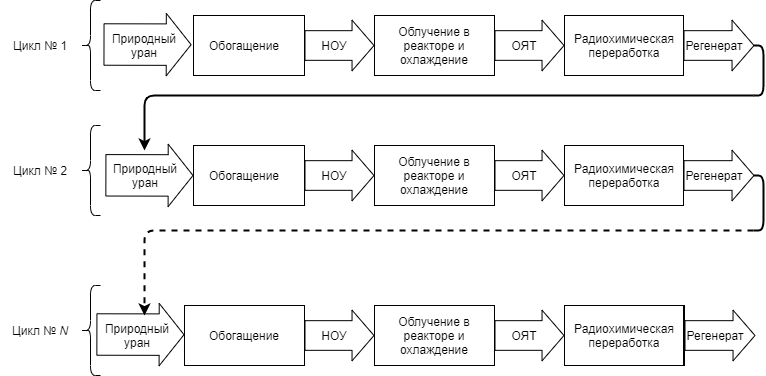
\includegraphics[scale=0.55]{theory/recycling_ru}}
  \caption{Схема многократного рециклирования урана}\label{recycle}
\end{figure}

В ходе рециклирования происходит монотонный рост концентраций четных изотопов в регенерате после облучения в реакторе. При этом ввиду относительной малости концентрации $^{232}$U на первом (или, в некоторых случаях, на первых двух) рециклах и, как следствие, не достижения концентрацией этого изотопа предельных значений в финальном продукте (товарном НОУ) для данных рециклов наблюдается наиболее резкий рост концентраций четных изотопов. Последующий постепенный выход на «плато», начиная с $\approx$3-го рецикла, очевидно, обусловлен фиксацией концентрации изотопа $^{232}$U в продукте на уровне $5\cdot10^{-7}$\%, что требует более сильного разбавления регенерата.

Это обстоятельство делает актуальным разработки каскадных обогатительных схем, позволяющих эффективно использовать регенерированный уран при производстве товарного НОУ с учетом всех описанных выше требований и ограничений как в условиях многократного рецикла урана.

\section{Промышленный опыт}\label{sec:ch1/sec1}

Возврата уран в топливный цикл по представленной выше схеме опирается на три ключевые технологии:
\begin{enumerate}
  \item ридиохимическую переработку ОЯТ;
  \item изотопное обогащение регенерированного урана;
  \item фабрикацию топлива на основе восстановленного отработавшего топлива.
\end{enumerate}

Что касается первого пункта, в мире в странах лидирующих в развитии ядерных технологий с середины прошлого века широко используется технология гидрометаллургической переработки облученного топлива, называемая PUREX \cite{selvaduraySurveyNuclearFuel1979}. В России, технологии связанные с переработкой ОЯТ развиваются особенно успешно благодаря ориентированности отрасли на замыкание ЯТЦ \cite{balihinSostoyaniiPerspektivahRazvitiya2018, efimenkoProblemyPerspektivyRazvitiya2017}. В виду такого стратегического курса отечественной атомной отрасли, запланирован ввод новых мощностей, которые расчитаны на переработку принимаемого ОЯТ из-за рубежа \cite{050519L3942005}

Что касается второго пункта, технологии изотопного обогащения урановых смесей, российская атомная промышленность имеет опыт обогащения регенерированного урана из реакторов ВВЭР-440, который затем использовался в качестве топлива РБМК \cite{VVER10001200Za}. Такая схема реализована для производства исходного сырья для изготовления топлива РБМК на заводе РТ-1 \cite{volkVozvratUranaIz2010}. Этот вариант также апробирован для изготовления опытных тепловыделяющих сборок (ТВС) для реакторов ВВЭР, требующих более высокого уровня обогащения \cite{proselkovAnalizVozmozhnostiIspolzovaniya2003}. Здесь важно также отметить, что на сегодняшний день у топливного дивизиона Росатома имеется уникальный технологический задел, связанный с газоцентрифужной технологией, который уже сегодня отражен в доминирующей роли этой технологии на мировом рынке разделительных услуг за счет низкой себестоимости единицы работы разделения, которую обеспечивают энергоэффективные и долговечные разделительные аппараты.

Что касается заключительного пункта пункта, Росатом на одном из заводов фабрикации ядерного топлива проводил испытания фабрикации тепловыделяющих сборок в том числе на основе зарубежного облученного топлива (из Франции) с повышенным содержанием $^{232}$U \cite{kislovRadiacionnyeAspektyIspolzovaniya}.

Также в россии имеется опыт возврата топлива в ЯТЦ базируется на смешении регенератов урана, извлекаемых из ОЯТ ВВЭР и ОЯТ транспортных реакторов с высоким содержанием $^{235}$U \cite{international2003iaea}.

При этом зарубежный опыт исторически базируется на однократном использовании MOX-топлива \cite{international2003iaea}.


% При этом, опираясь на передовой уровень разделительной технологии, можно заключить, что задача обогащения регенерата до необходимого для повторного использования в энергетических ядерных реакторах уровня концентрации изотопа $^{235}$U может быть решена.

Таким образом, сложившаяся к текущему моменту научно-производственная база и лидирующие объемы имеющихся в нашей стране промышленных разделительных мощностей, основанных на центробежном методе разделения, являются основным аргументом в пользу готовности к вовлечению регенерата в топливный цикл легководных реакторов.

Однако, для практической реализации долгосрочных планов отрасли по замыканию ЯТЦ и расширению предложения международных топливных поставок, что предусматривает необходимость многократного рецикла, необходимо решить задачу возврата регенерата в ЯТЦ, подразумевая наличие вышеизложенных ограничений.

Для анализа теоретической возможности решения задачи рецикла урана в рамках поставленных ограничений с помощью ранее предложенных схем, перейдем к их подробному рассмотрению.

\section{Сравнительный анализ известных схем}

История теоретических исследований вопроса повторного использования урана в ядерном топливе насчитывает около полувека.
В этом разделе будет рассмотрена эволюция способов, предложенных для решения задачи обогащения регенерированного урана с целью его возврата в топливный цикл энергетических реакторов.
Развитие подходов к вовлечению регенерата в производство низкообогащенного урана можно проследить через историю совершенствования предлагаемых каскадных схем.
Для каждой рассмотренной схемы будет проведен критический анализ, выявляющий ее достоинства и недостатки.

\subsection{Базовые модификации ординарного каскада}

Непосредственное применение простейшей схемы -- ординарного каскада, используемого для обогащения природного урана имеет существенные ограничения в рамках поставленной нами задачи.

Рассмотрим же технические решения, позволяющие, соблюдая вышеозначенные условия, решить задачу обогащения регенерата. Начнем с ряда схем, основанных на ординарном (трехпоточном) каскаде.
Его можно применять, например, следующими способами (рис. \ref{fig:diagram1}) \cite{sulaberidzeNekotoryhRazdelitelnyhProblemah2004,smirnovKaskadnyeShemyZadachah2012}:
\begin{enumerate}
  \item Добавление смеси регенерированного урана к природному урану перед подачей в каскад рис. (рис. \ref{fig:diagram1}.1).
  \item Получение обогащенной фракции из регенерата и последующее ее разбавление природной урановой смесью (рис. \ref{fig:diagram1}.2 ).
  \item Подготовка смеси НОУ из природного урана немного больше, чем необходимо для получения товарного НОУ требуемого качества, с последующим разбавлением его регенератом (рис. \ref{fig:diagram1}.3 ).
\end{enumerate}

\begin{figure}[ht]
  \centerfloat{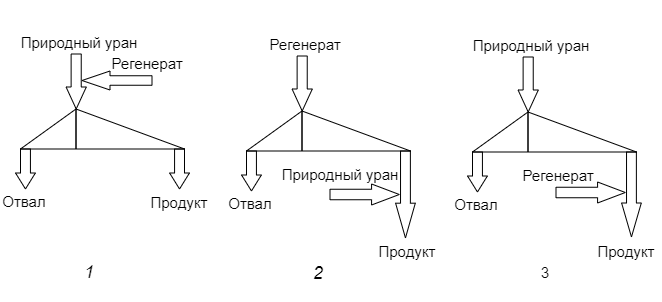
\includegraphics[scale=0.7]{cascades/diagram1}}
  \caption{Схемы на основе ординарного каскада}\label{fig:diagram1}
\end{figure}

Для всех вариантов схем рис. \ref{fig:diagram1} сотношение между расходом регенерата и разбавителем природного происхождения определяется пределом допустимой концентрации $^{232}$U в конечном продукте -- низкообогащенном уране. Также компенсируется отрицательная реактивность $^{236}$U с помощью добавочной концентрации $^{235}$U к той, что требуется для НОУ-топлива с заданными свойствами.

Основным преимуществом таких схем является простота реализации, поскольку нет необходимости в модификации устройства каскада -- операции разбавления осуществляются за пределами  ординарного каскада.
При этом, как недостаток можно выделить потери работы разделения, возникающие из-за смешения потоков с различными изотопными концентрациями $^{235}$U.

Рассмотрим вариант схемы, изображенный рис.\ref{fig:diagram1}.1. Принцип ее работы состоит в предварительном смешении регенерата с природным ураном перед подачей результирующей смеси на питание каскада, в котором будет получен конечный НОУ-продукт. А пропорция смешения этих исходных питающих смесей определяется из ограничения на $^{232}$U в конечном НОУ-продукте, и с поправкой на необходимость компенсации $^{236}$U в обогащенном продукте дополнительным количеством делящегося $^{235}$U.

Вариант схемы, изображенный рис.\ref{fig:diagram1}.2 представляет другой возможный способ снижения накопления четных изотопов в регенерате урана \cite{SposobIzotopnogoVosstanovleniyaa}. Разбавление осуществляют следующим образом: сначала из регенерата в ординарном каскаде получают высокообогащенный уран (ВОУ), который затем разбавляют смесью, не содержащей минорных изотопов -- природным ураном, добиваясь нужного содержания изотопа $^{235}$U в финальном продукте-низкообогащенном уране. На месте разбавителя в виде природного урана может также быть и изотопная смесь на основе природного урана, не содержащая изотопов искусственного проихождения $^{232,236}$U, так как главной целью является разбавление этих изотопов, имеющихся в регенерированном уране.

Также существует вариант схемы, изображенный рис.\ref{fig:diagram1}.3, где предварительно обогащенный природный уран смешивается с возвращаемым в топливный цикл регенерированным ураном. К получаемому продукту на основе этих двух материалов предъявляются аналогичные требования, что определяет пропорции смешения изотопных составов и уровень обогащения природного урана.

Практическое использование данной схемы ограничивают следующие недостатки (количественные оценки для рассматриваемой схемы будут представлены во второй главе): 
\begin{enumerate}
  \item потери работы разделения при разбавлении ВОУ.
  \item увеличение радиационного фона на производстве из-за загрязненности разделительного оборудования примесными изотопами, в частности $^{232}$U.
  \item для рассмотренного случая производства НОУ-топлива для легководных реакторов, необходимость обогащения материала до уровня высокообогащенного урана, когда концентрация изотопа $^{235}$U превышает 20\%.
  Такой подход может иметь ограничения со стороны регулятора -- обогатительный комбинат может быть не в праве нарабатывать материал с такой высокой концентрацией $^{235}$U -- в соответствии с режимом нераспространения \cite{brownOriginsSignificanceLimit2016}.
  \item невозможность обеспечить полный возврат ОЯТ в ЯТЦ в условиях многократного рецикла. Добиться желаемого результата невозможно ввиду наличия ограничений на присутствие в конечном продукте -- низкообогащенном уране -- четных изотопов. Это было показано в работах \cite{sulaberidzeNekotoryhRazdelitelnyhProblemah2004,sulaberidzeProblemsRefinementRecycled4, smirnovKaskadnyeShemyZadachah2012} где было сделано заключение, что отрицательное влияние указанных изотопов делает непригодным для обогащения регенерата ординарный каскад (каскад, имеющий три внешних потока – питание, отбор и отвал), используемый для обогащения природного урана. Это происходит, поскольку при обогащении регенерата по $^{235}$U в таком каскаде, в отборе, помимо $^{235}$U неминуемо будут концентрироваться все легкие компоненты, в первую очередь $^{232}$U.
\end{enumerate}

Поэтому ординарный каскад применим только для обогащения относительно «чистого» состава регенерата, в котором содержание $^{232}$U меньше допустимой нормы на порядок и более, что нехарактерно для большинства изотопных составов выгружаемого из активной зоны ВВЭР облученного топлива \cite{bormanTehnikoekonomicheskiyAnalizVozmozhnyh2012}. Такое ограничение и подтолкнуло исследователей к развитию подходов к производству НОУ из обогащенного регенерата с учетом заданных требований. Однако, следует помнить, что ординарные трехпоточные каскады могут быть использованы в качестве составных элементов для усовершенствованных каскадных схем, с помощью которых будет возможно решить поставленную задачу с выполнением всех условий.

Как будет доказано во второй главе, использование базовых модификаций ординарного каскада не целесообразно для решения задачи возврата в ЯТЦ регенерированного урана в условиях многократного рецикла, даже если пренебречь нормативным ограничением на производство ВОУ.
Таким образом, рассмотрение приведенного ряда модификаций ординарного каскада подталкивает к дальнейшим поискам схем, которые бы нивелировали перечисленные недостатки.

\subsection{Каскады с дополнительными внешними потоками (многопоточные схемы)}

Ниже дан критический анализ модификаций каскадных схем для обогащения регенерированного урана, основанных на использовании одиночных каскадов, имеющих дополнительные внешние потоки.

Под внешними потоками следует понимать потоки, подаваемые в качестве питания каскада, и выходящие из каскада потоки, а под внутренними -- потоки, циркулирующие внутри каскада. 

При подаче дополнительного независимого потока в каскад, основной поток питания, содержащий разделяемые компоненты, подается в точку питания $f$(на вход ступени с номером $f$), а дополнительный поток питания -- в точку питания $l$ (на вход ступени с номером $l$). В случае условия несмешивания концентраций $^{235}$U при подаче питающего потока, дополнительный поток с концентрацией $^{235}$U подается в ступень, подбираемую следующим образом: концентрация целевого компонента в питающем потоке должна соответствовать его концентрации в принимающей ступени.

Подключение же дополнительного отбора осуществляется на том участке каскада, где необходимый для изъятия из каскада компонент локализуется.

\subsubsection{Использование дополнительного потока-разбавителя}

В \cite{sulaberidzeQuasiidealCascadesAdditional2006} предожена схема с дополнительным потоком питания в виде регенерата, который подают на отдельную внутреннюю ступень каскада (рис. \ref{fig:2_inputs}).
\begin{figure}[ht]
  \centerfloat{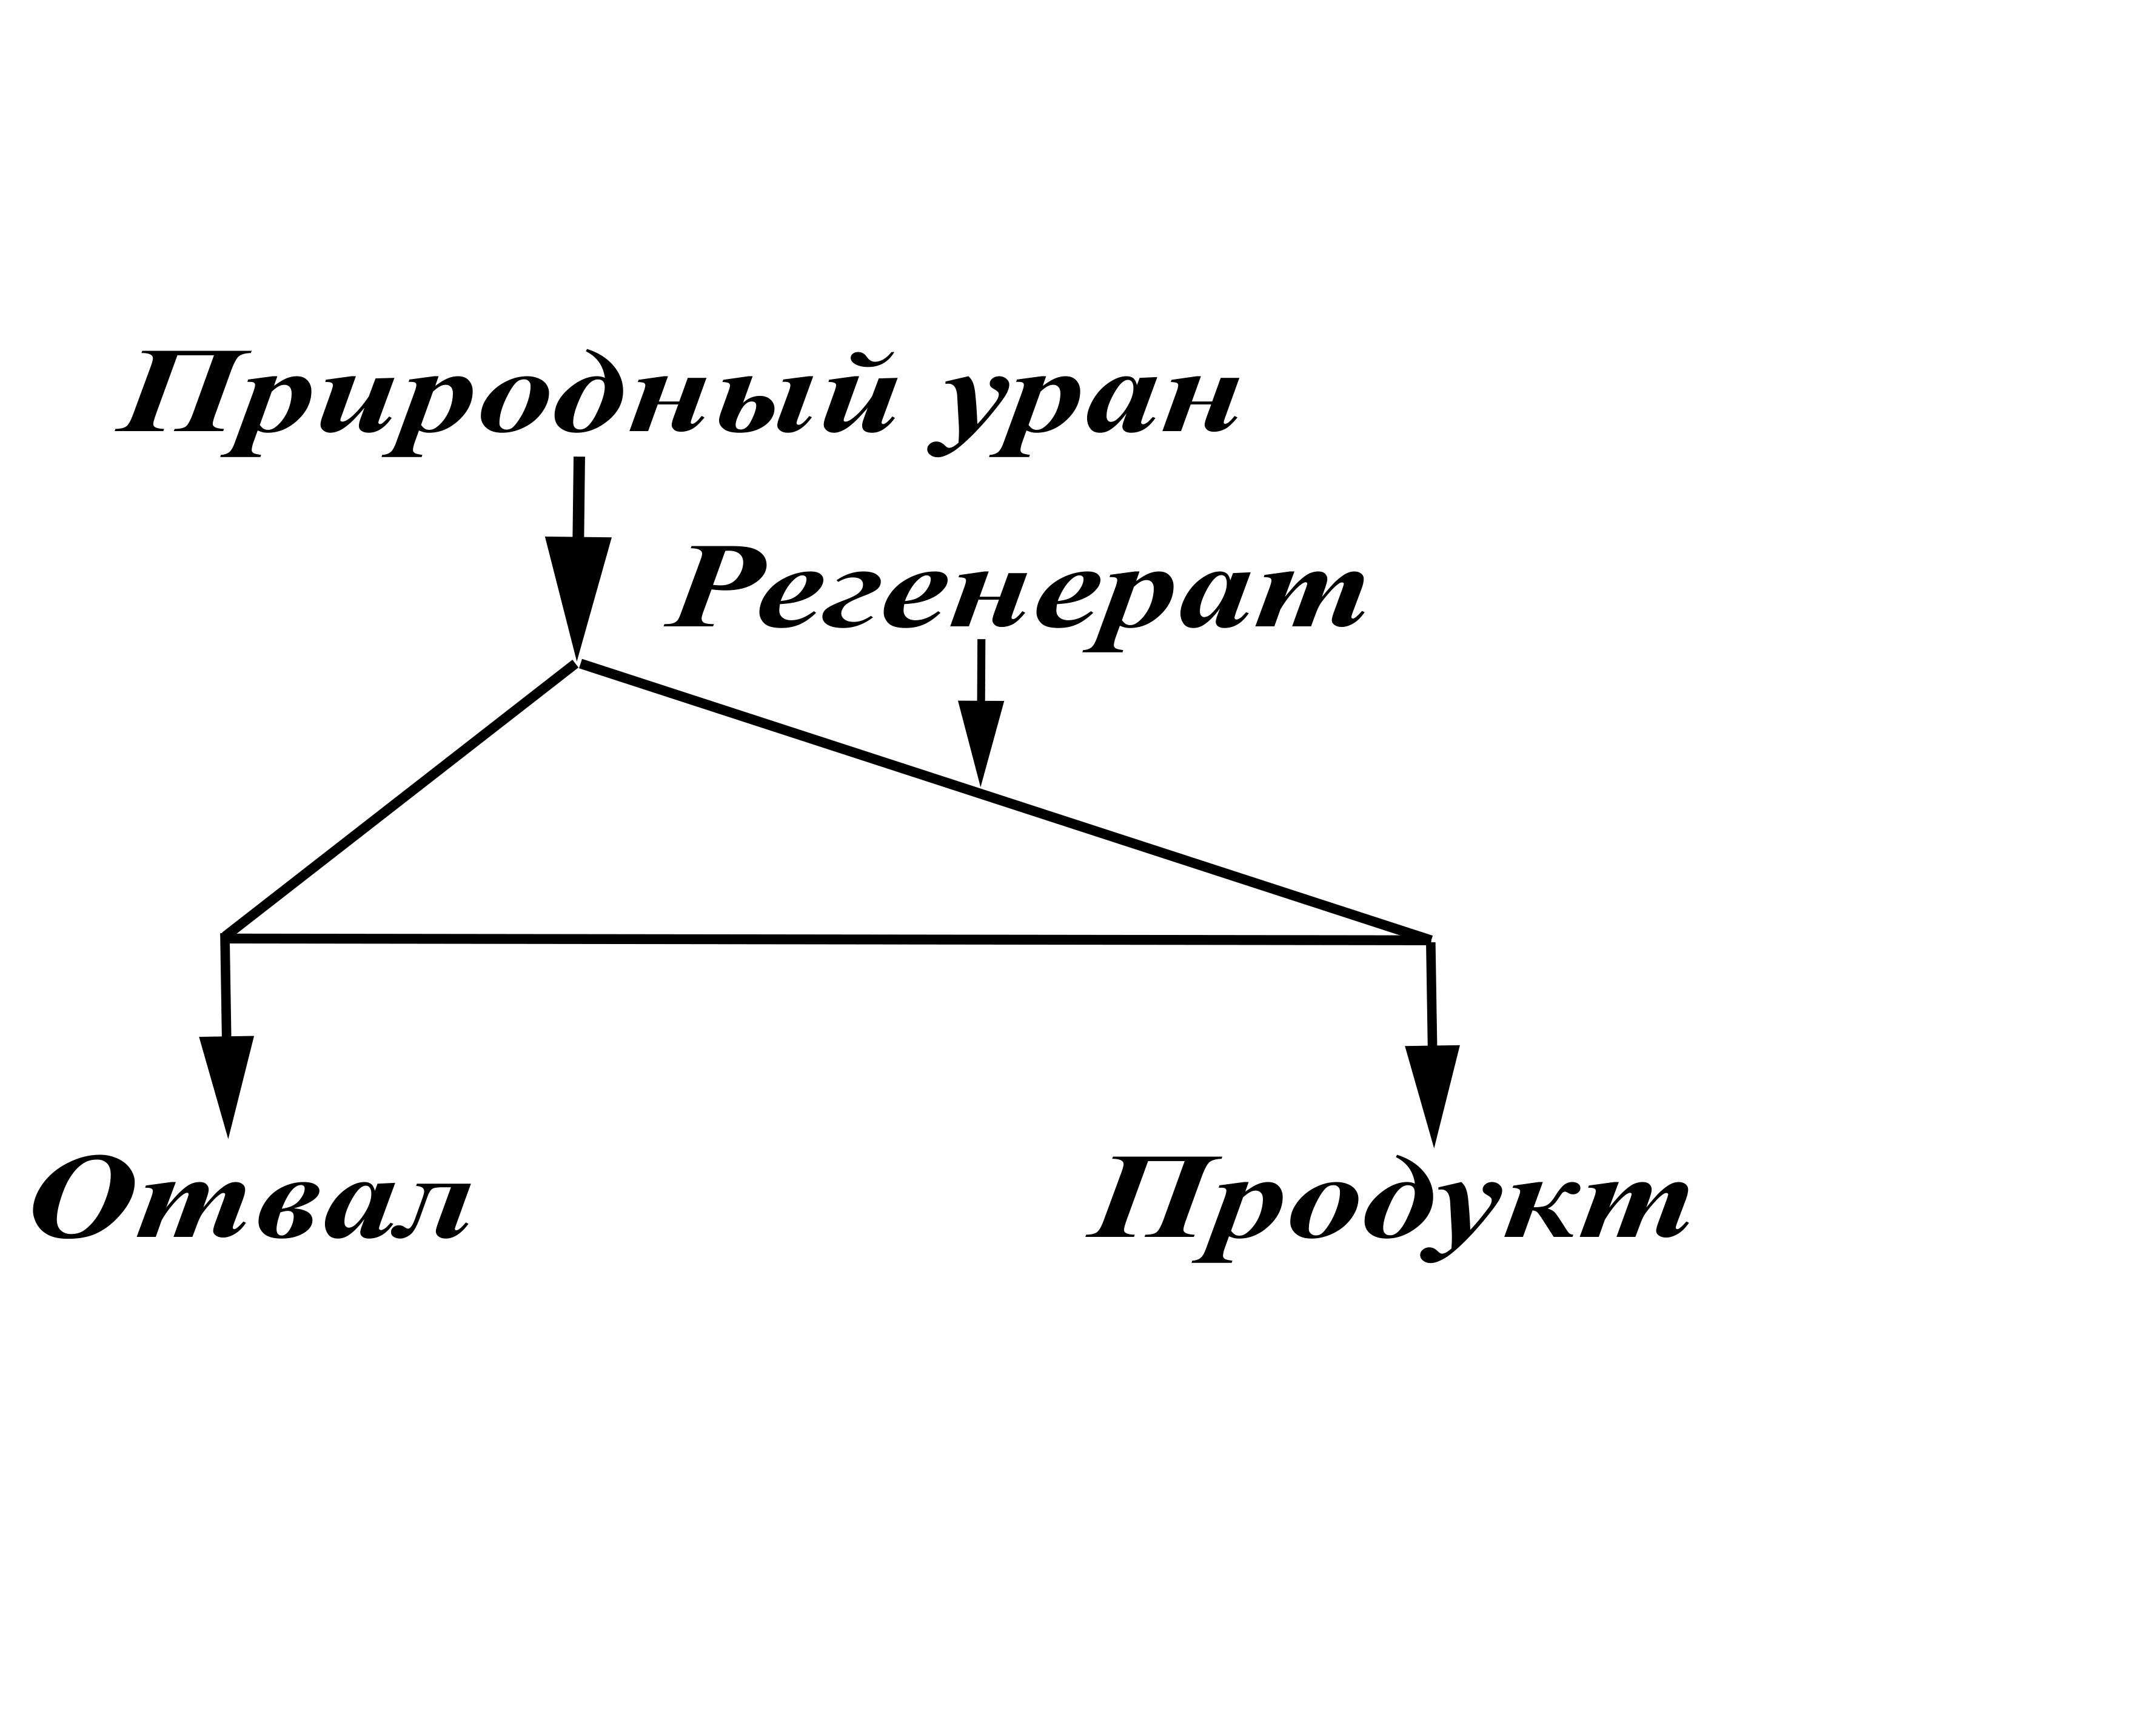
\includegraphics[scale=0.07]{cascades/2in}}
  \caption{Каскад с дополнительным потоком питания}\label{fig:2_inputs}
\end{figure}

Этот метод позволяет схеме с дополнительным потоком питания избежать потери работы разделения в ходе смешения потоков с различными концентрациями $^{235}$U, располагая дополнительный входной поток там, где концентрации внешнего и внутреннего потоков в $^{235}$U совпадают \cite{smirnovKaskadnyeShemyZadachah2012, sulaberidzeQuasiidealCascadesAdditional2006}.

Однако общим недостатком всех вышеупомянутых схем (рис. \ref{fig:diagram1} и \ref{fig:2_inputs}), является необходимость осуществления разбавления регенерата существенным количеством природного урана, в несколько раз превышающим долю используемого регенератадля снижения содержания $^{232}$U в продукте.
Тем не менее, при повторном использовании регенерированного урана из топлива ВВЭР, даже такой подход может обеспечить значительную экономию природного урана ($\approx$16\% согласно \cite{alekseevPossibleScenariosTransition2020}).
Суммарная же экономия природного урана за всю серию рециклов будет складываться из уменьшающихся с каждым рециклом показателей сэкономленного природного сырья \cite{colemanEvaluationMultipleSelfrecycling2010,smirnovEvolutionIsotopicComposition2012}).

Проблема необходимости обеспечивать питание каскада преобладающим количеством природного урана, чтобы, в сущности, «разбавлять» четные изотопы  $^{232,234}$U, содержащиеся в регенерате, идет бок о бок с невозможностью обеспечить условие полного возврата ОЯТ в ЯТЦ, то есть использования 1 кг ОЯТ на 1 кг НОУ продукта. 
Это условие необходимо для полного замыкания цикла по урану и, тем самым, корректного контроля за оборотом делящихся материалов при экспортных поставках топлива. С другой стороны, в условиях российской ядерной энергетики оно позволяет не создавать складской запас регенерированного урана, хранение которого требует определенных затрат.


Выполнение такого условия достижимо только для изотопных составов первого (иногда второго) рецикла топлива легководного реактора.
Таким образом, с помощью такой схемы нельзя обеспечить заданную пропорцию вовлечения регенерированного урана в условиях многократного рецикла, так как, начиная с третьего цикла, расходовать требуемый уровень регенерата становится невозможно из-за ухудшения изотопного состава урана и наличия ограничений на изотопы $^{232,236}$U \cite{smirnovApplyingEnrichmentCapacities2018}.

Так, в \cite{smirnovApplyingEnrichmentCapacities2018} были рассчитаны основные показатели, характеризующие экономику производства обогащенного урана: расход природного урана и затраты работы разделения (РР).
Было показано, что для каждого из первых двух циклах можно достичь экономии природного урана на уровне $\approx$20\%. Затем, этот показатель ухудшается, так как при заданных условиях, к третьему циклу повторного использования происходит значительная деградация изотопного состава, заключающаяся в накоплении в урановой фракции нежелательных четных изотопов $^{232,234,236}$U, которые не поддаются извлечению радиохимическими технологиями.
Чтобы повысить пределы экономии природного урана, необходимо искать альтернативный разбавитель. Например, таким материалом может послужить обедненный уран (так называемые «хвосты» (или отвалы) -- побочный продукт процесса обогащения), который благодаря современным разделительным технологиям стало возможно использовать как ресурс делящегося $^{235}$U \cite{oecdManagementDepletedUranium2001, ITOGIDEYaTELNOSTIGOSUDARSTVENNOY}.
И это, только лишь за счет возможностей обогатительных производств, не говоря о перспективах наработки плутония из ОГФУ в быстрых реакторах.

% Для отечественной ядерной индустрии, $^{235}$U из <<богатых>> источников ОГФУ ($\approx$0.3\%), является важным источником сырья для производства ядерного топлива, а также доходным международным бизнесом \cite{oecdManagementDepletedUranium2001}.
% Имеющиеся в мире запасы $\approx$1.2 миллиона тонн <<богатых>> хвостов (0.3\%) дают эквивалент 336 тысяч т. эквивалента природного урана при концентрации $^{235}$U в отвале 0.14\%. Этого достаточно, чтобы обеспечить на 5 лет топливом весь мировой парк энергетических реакторов.
% Стоит отметить, что наличие ОГФУ такой категории связано с историей развития обогатительного производства. Ввиду того, что диффузионный метод разделения -- технология первого поколения -- требует колоссальных затрат энергии на единицу РР, получение обогащенного продукта было целесообразней осуществлять с б'ольшими затратами природного урана.
% Напомним, что выбор в пользу затрат на каждый из этих показателей связан с компромиссом, определяемым, во многом, экономическими факторами: себестоимостью единицы работы разделения и стоимостью сырья. 
% Итак, согласно годовому отчету ГК <<Росатом>> 2019 г. (стр. 45 \cite{ITOGIDEYaTELNOSTIGOSUDARSTVENNOY}), поставки из вторичных источников (складские запасы энергокомпаний и некоторых государств, дообогащение обедненного гексафторида урана, регенерированный уран и пр.) оцениваются на уровне 20 тыс. т в эквиваленте природного урана.

Перейдем к описанию каскада, позволяющего задействовать ОГФУ в повторном обогащении регенерированного урана.
Такая схема изображена на рис. \ref{fig:3_inputs}, где $F_{1}, F_{2}, F_{3}$ -- потоки питания в виде ОГФУ, природного урана и регенерата, соответственно; а $W$ и $P$ -- потоки отвала и питания.
Основной принцип устройства данной схемы состоит в том, что входные потоки располагают там, где концентрация изотопа $^{235}$U во внешнем (питание каскада) и внутреннем потоках (в ступени каскада) совпадают.
Подробное описание математической модели приведено в \cite{smirnovEnrichmentRegeneratedUranium2014}.

\begin{figure}[ht]
  \centerfloat{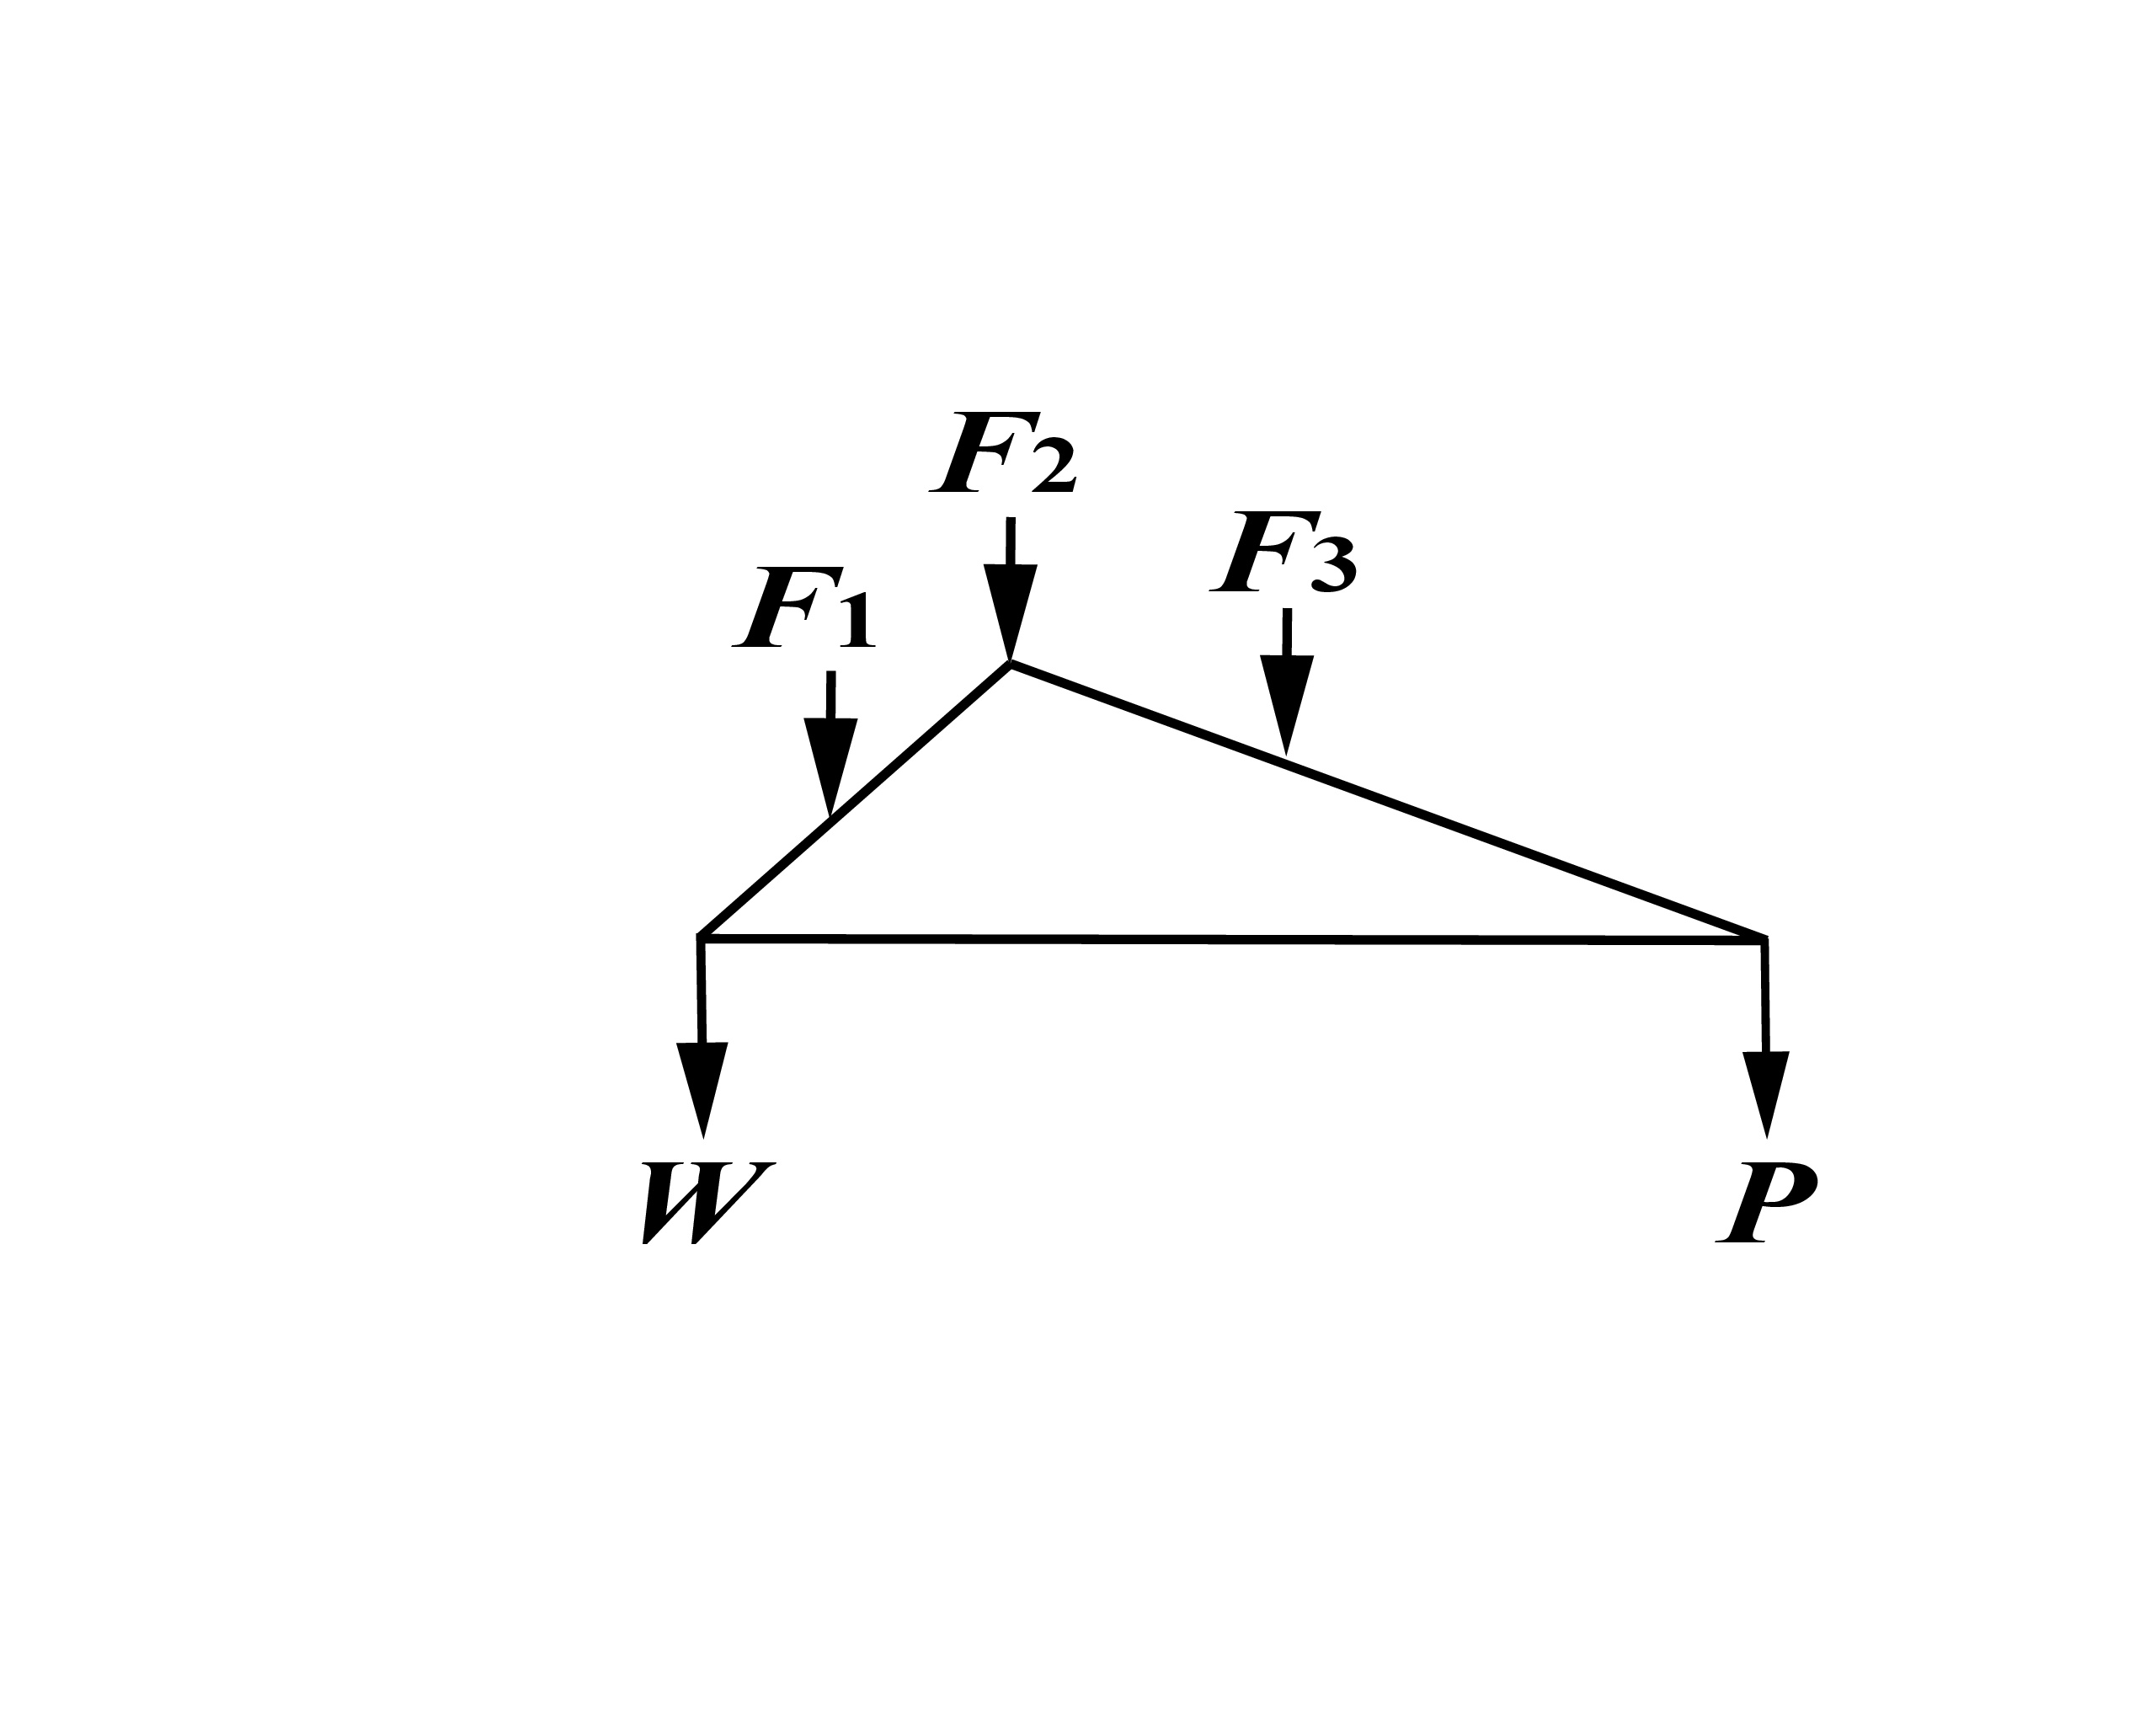
\includegraphics[scale=0.17]{cascades/3in}}
  \caption{Каскад с тремя потоками питания}\label{fig:3_inputs}
\end{figure}

Преимущества схемы рис. \ref{fig:3_inputs}:

\begin{enumerate}
  \item возможность настраивать каскад для достижения компромисса между показателями экономии природного урана и расхода работы разделения, то есть осуществлять регулировку интегральных характеристик разделительного процесса. Такой прием может позволить добиваться оптимального по себестоимости баланса затрат на эти два конкурирующих показателя. Например, в работе \cite{smirnovApplyingEnrichmentCapacities2018}, демонстрируется экономия половины природного урана на каждом рецикле.
  \item частичное решение проблемы утилизации накопленных объемов обедненного урана \cite{smirnovEnrichmentRegeneratedUranium2014}. Поскольку гексафторид урана является агрессивным веществом, его хранение связано с затратами, и емкости для хранения следует время от времени заменять из-за коррозионных процессов \cite{fitchOPTIONSDISPOSALREAPPLICATION2009, oecdManagementDepletedUranium2001}.
\end{enumerate}

Однако следует отметить, что этот подход предполагает снижение содержания $^{235}$U в образовавшемся ОГФУ, по сравнению с исходным, и требует исследования перспектив дальнейшего использования такого материала в бланкетах реакторах-бридерах \cite{smirnovApplyingEnrichmentCapacities2018}.
Произведенный посредством схемы рис. \ref{fig:3_inputs} дважды обедненный ОГФУ, к тому же содержащий повышенную концентрацию минорных изотопов, по-видимому, должен быть первым на очереди к переводу в стабильную форму. Такая переработка, заключающаяся в обеcфторивании и переводе в закись-окись урана, осуществляется на установках типа «W-ЭХЗ» \cite{PererabotkaOGFUObrazovaniem2014}.

Итак, исходя из результатов работы \cite{smirnovApplyingEnrichmentCapacities2018}, схема (рис. \ref{fig:3_inputs}), как и схема рис. \ref{fig:2_inputs}, для заданных составов, характерных современным ВВЭР, позволяет обеспечить полный возврат урана в ядерный топливный цикл только для двух первых рециклов урановой компоненты из-за быстрого накопления четных изотопов  $^{232,234,236}$U, от которых в такой схеме невозможно произвести очистку, выводя легкие изотопы из системы $^{232,234}$U.

Важность сдерживания накопления $^{232}$U при многократном переиспользовании была показана в работе \cite{smirnovEvolutionIsotopicComposition2012}. Введение ограничения на $^{232}$U позволяет замедлить рост концентрации $^{236}$U в изотопном составе рециклируемого топлива.

Анализ перечисленных выше работ позволяет поставить проблему очистки изотопных составов от четных изотопов, которые имеют тенденцию накапливаться от рецикла к рециклу, приводя к ухудшению изотопного состава за счет накопления в нем изотопов $^{232,234,236}$U.

Однако, как было отмечено, во всех рассмотренных схемах заметное снижение содержания изотопов $^{232,234,236}$U в финальном НОУ достигается, прежде всего, за счет разбавления регенерата внутри каскада смесями, полученными из урана природного состава (НОУ, ОГФУ).

Отсюда возникает вопрос очистки изотопного состава рециклируемого материала от четных $^{232,234,236}$U, чтобы сдержать их накопление от рецикла к рециклу.

В качестве дополнительного аргумента для поиска альтернативных каскадов, позволяющих выводить из системы $^{232,234,236}$U, приведем следующий факт.
В последнее время конструкция ВВЭР развивалась к увеличению максимального выгорания топлива (до 70 $\frac{МВт*сут.}{кг}$ U в ВВЭР-1200) \cite{asmolovNewGenerationFirstofthe2017}, с целью снижения стоимости топливной составляющей \cite{andrianovaPovyshenieVygoraniyaTopliva2008}.
А так как, согласно природе цепной реакции, рост остаточного содержания $^{232,234,236}$U пропорционален уровню выгорания \cite{VeryHighBurnups2006}, схемы, нацеленные на очистку $^{232,234,236}$U представляются в будущем более перспективными.

% К тому же, в случае успеха в продвижении российских услуг по реконверсии RepU на мировом рынке, очистка от $^{232}$U может быть востребована в силу ограничения лицензии российского оператора ($5\cdot10^{-7}$\% (5ppb) по $^{232}$U), если не будут применены иные способы улучшения изотопного состава.
% Однако существуют практики возврата регенерата в ЯТЦ, для которых проблема очистки регенерата от четных $^{232,234}$U не актуальна вне необходимости многократного рецикла. Так, Французская электроэнергетическая компания EDF выбрала стратегию прямого обогащения регенерированного урана. Такой подход воплощен на АЭС Cruas, которая имеет лицензию на работу с топливом, в котором ограничение содержания $^{232}$U в 6 раз выше ограничения, принятого в РФ, и составляет 30 ppb.

Перечислим не связанные с разбавлением регенерата способы, с помощью которых можно частично удалить нежелательные изотопы из системы.

Такие способы непосредственно связаны со схемами, которые позволяют извлекать промежуточный продукт, или с помощью составных схемам (несколько последовательных каскадов, например, двойной каскад).

\subsubsection{Каскад с двумя питаниями, одним отвалом, основным и дополнительным отбором}
Схемы, называемые каскадами с промежуточным продуктом были предложены с целью «очистки» от четных изотопов $^{232,234,236}$U параллельно с производством основного НОУ-продукта (рис. \ref{fig:3_out}) \cite{zhurinSPOSOBPERERABOTKIZAGRYaZNENNOGO, palkinAnaliticheskiyRaschetSoderzhaniya2007}. В качестве материалов, которые необходимо очистить от изотопов $^{232,234,236}$U посредством такой схемы, помимо регенерированного урана, можно рассматривать составы загрязненного урана природного состава, а также «хвостов» процесса обогащения \cite{palkinSeparationUraniumIsotopes2010}. 

Здесь в качестве основного продукта получают НОУ требуемых характеристик, а в качестве промежуточного продукта получают состав с пониженным содержанием нежелательных изотопов.
\begin{figure}[ht]
  \centerfloat{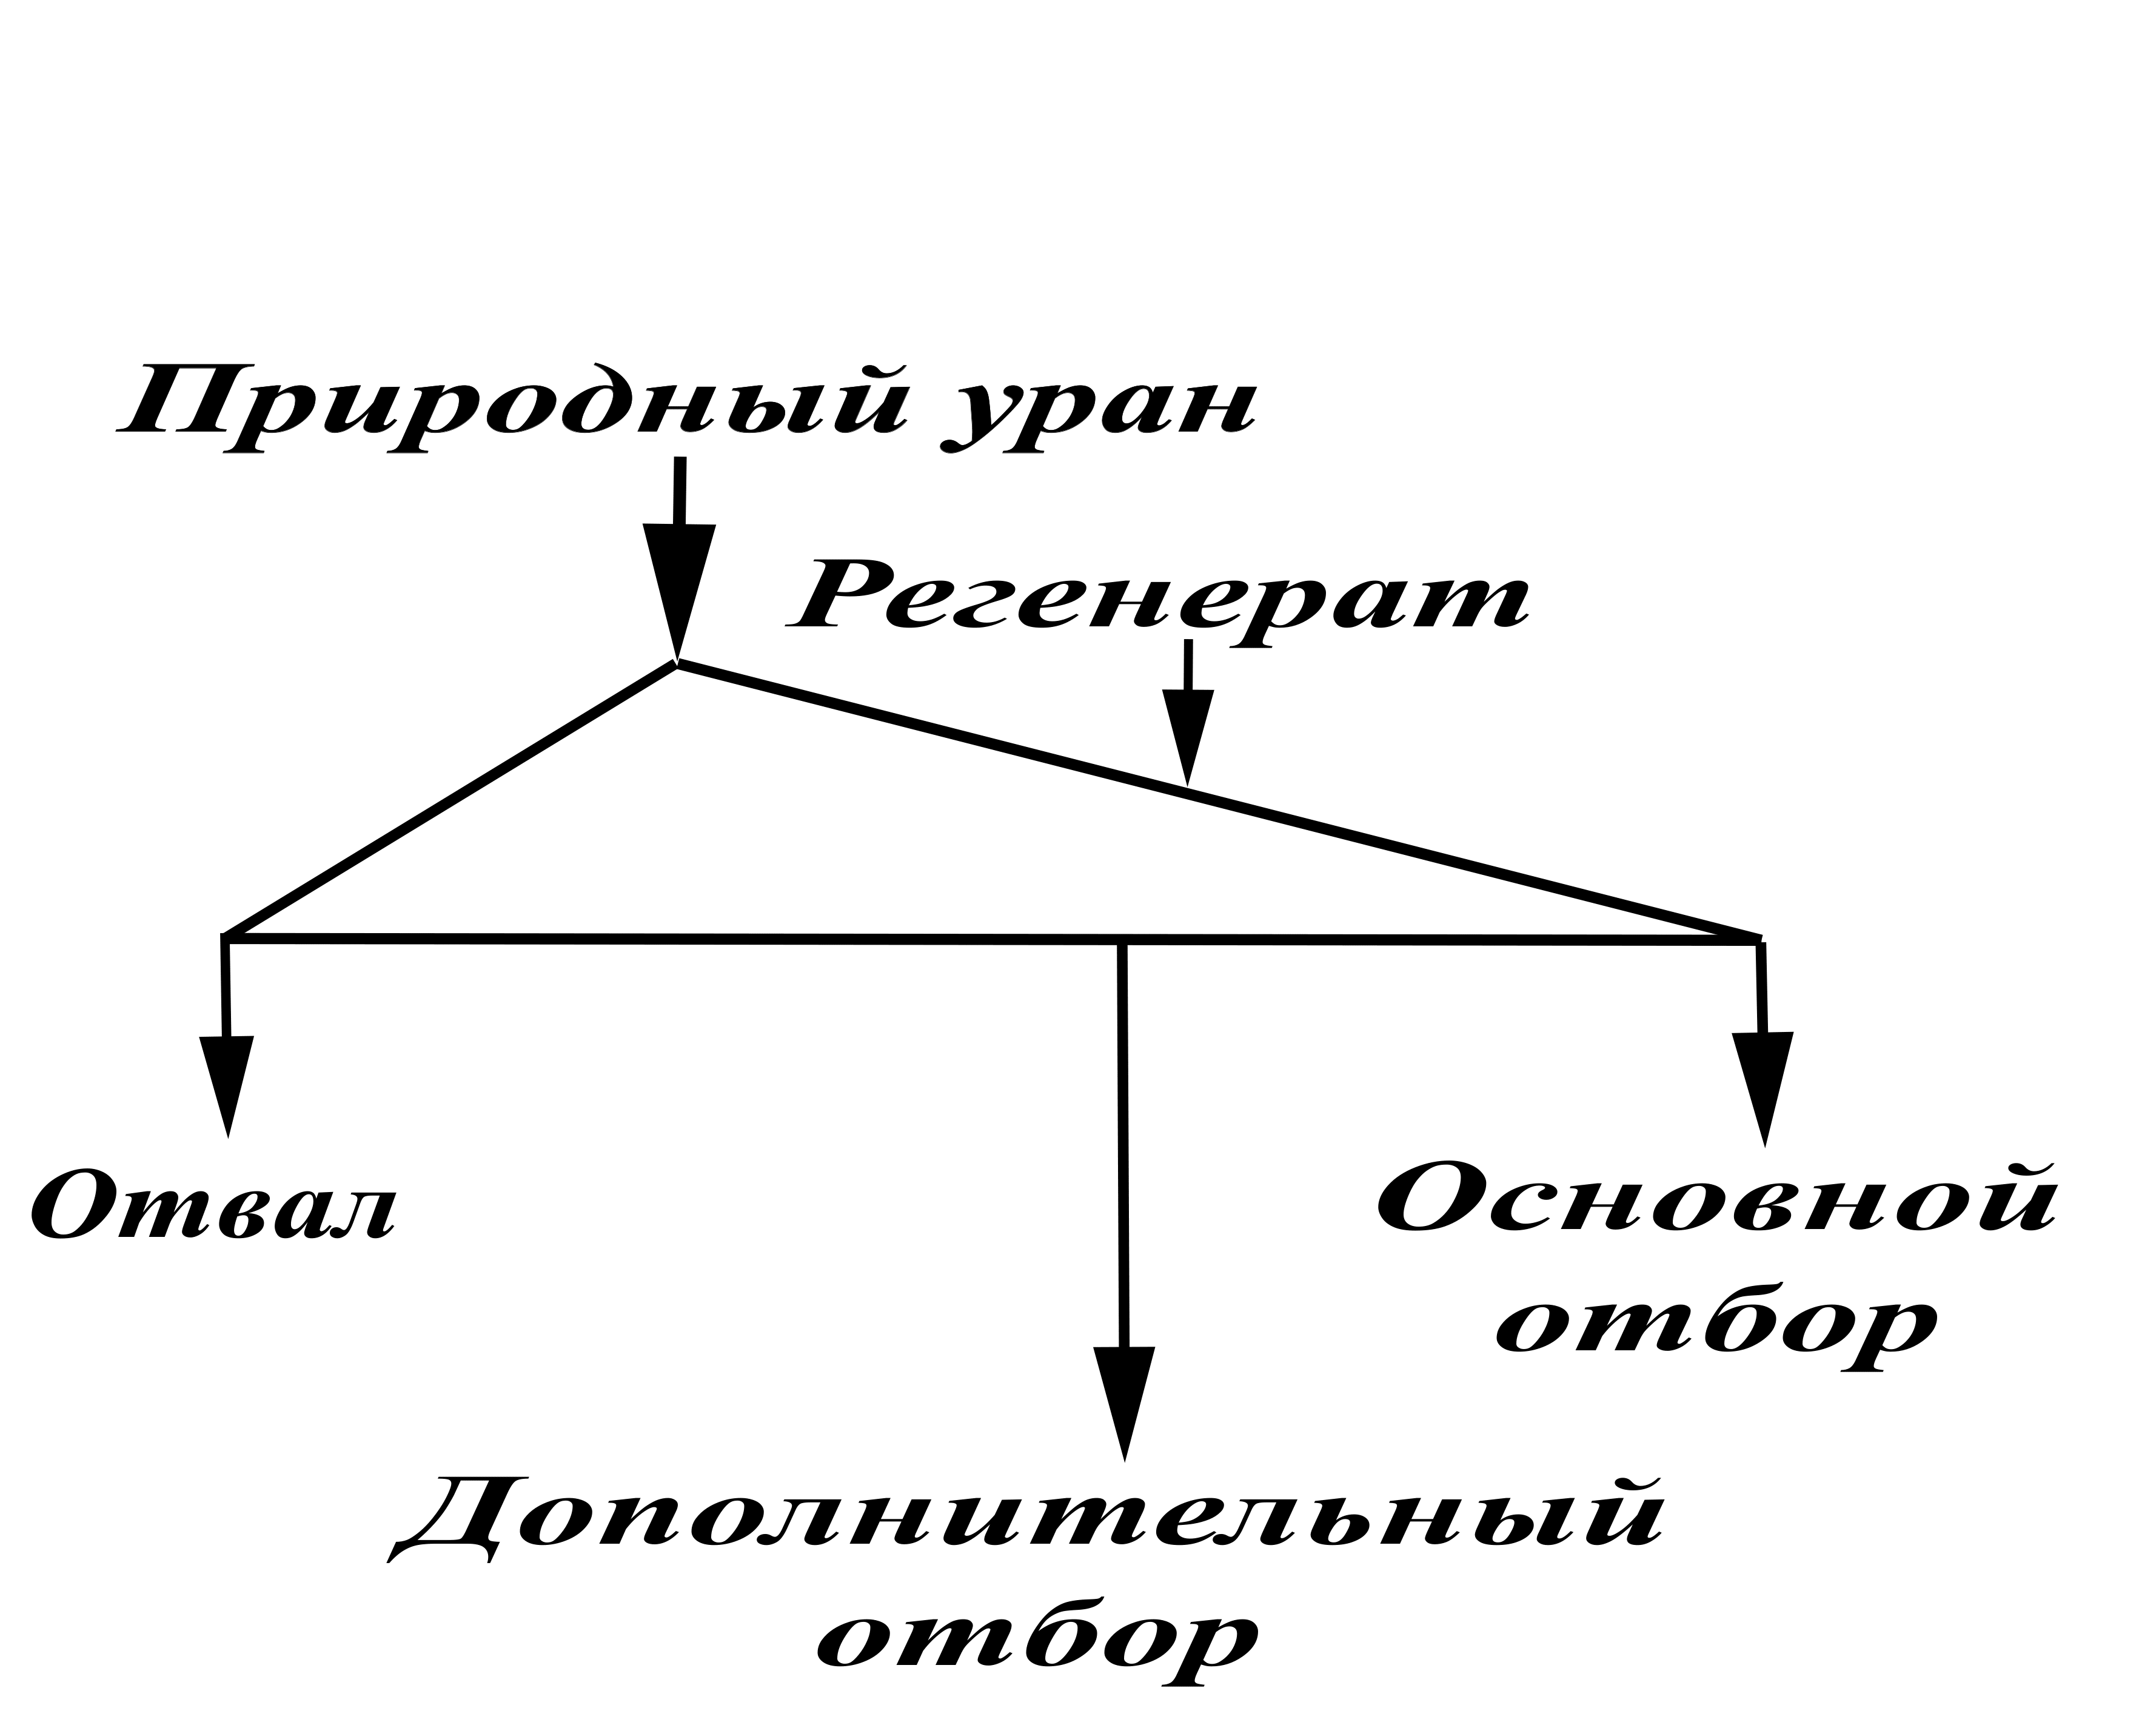
\includegraphics[scale=0.07]{cascades/3out}}
  \caption{Каскад с дополнительным потоком отбора}\label{fig:3_out}
\end{figure}

Получение в выходящем потоке дополнительного отбора смеси с пониженными концентрациями $^{232,234,236}$U и схожей с питающим регенератом концентрацией $^{235}$U, позволяет более эффективно использовать такой полупродукт для производства товарного НОУ \cite{palkinSeparationUraniumIsotopes2010}. Концентрация $^{235}$U в этом <<очищенном>> продукте подбирается так, чтобы она минимально отличалась от концентрации в потоке дополнительного питания в виде регенерата. Это позволяет при соблюдении эквивалентности этих потоков исключить потери работы разделения. В результате такой очистки исходного регенерата содержание всех четных изотопов значительно снижается. Низкообогащенный уран с концентрациями $^{232,234,236}$U, удовлетворяющими требования ASTM для коммерческого продукта, может быть получен из такого подготовленного промежуточного продукта путем его прямого обогащения \cite{shopenSposobPolucheniyaRazbavitelya2008}.

При этом важно заметить, что продукт, получаемый в потоке <<основной отбор>> такого каскада, сразу соответствует качеству товарного НОУ для легководных реакторов \cite{palkinSeparationUraniumIsotopes2010}. Однако, высокое качество очищенного регенерата достигается только при малой доле потока питающего регенерата относительно природного урана, если необходимо оставаться в рамках требований к НОУ, производимом в потоке основного отбора.

Подробнее такой подход рассмотрен в работе \cite{palkinPurificationReprocessedUranium2016}, где предложена схема, представленная на рис. \ref{fig:int_double}. Принцип ее работы состоит в следующем.

\begin{figure}[ht]
  \centerfloat{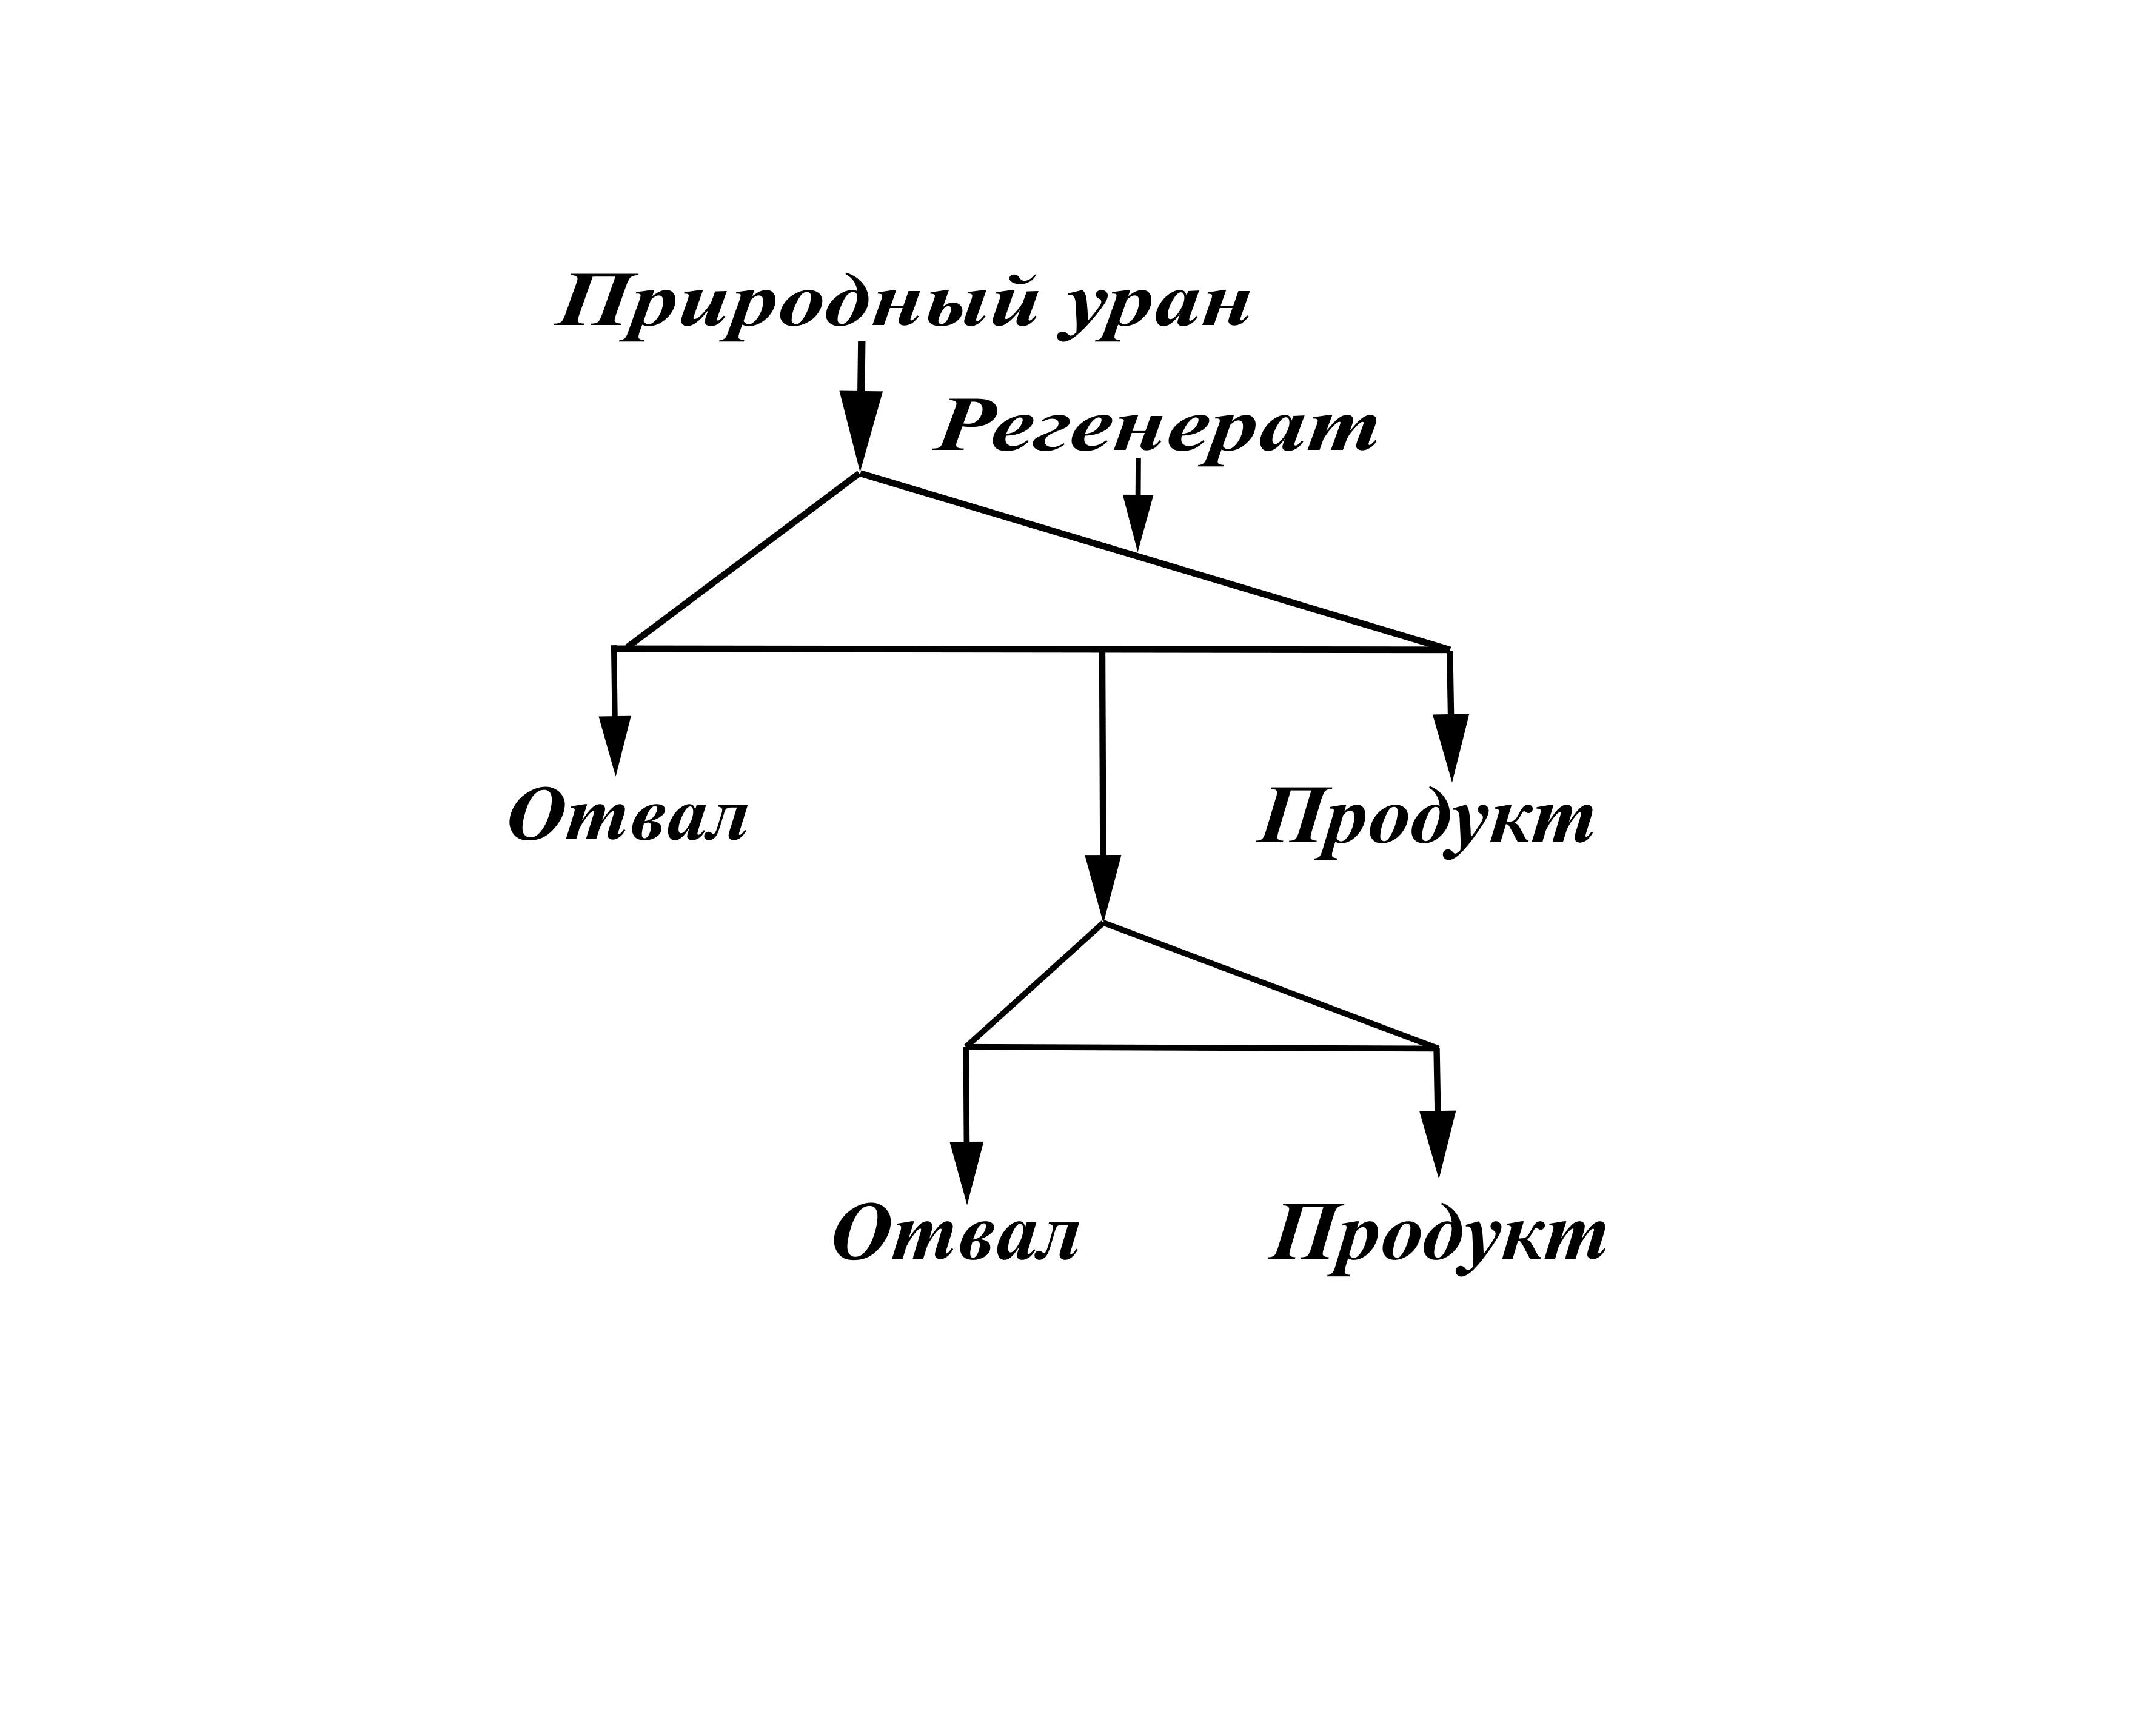
\includegraphics[scale=0.15]{cascades/int_double}}
  \caption{Двойной каскад на основе каскада, получающего очищенный регенерат}\label{fig:int_double}
\end{figure}

Очищенный полупродукт (дополнительный промежуточный отбор), полученный в первом каскаде, представленном выше (рис. \ref{fig:3_out}), поступает в следующий каскад, где обогащается до необходимого уровня по $^{235}$U. Такая схема предусматривает возможность значительного снижения нежелательной концентрации $^{236}$U в случае уменьшения потока дополнительного отбора -- промежуточного продукта первого каскада.
Этот эффект можно применить следующим образом: например, снизить концентрации  $^{234}$U и  $^{236}$U в промежуточном продукте (16\% для  $^{236}$U), при этом всего лишь незначительно уменьшив (всего на 4\%) поток этого полупродукта \cite{palkinPurificationReprocessedUranium2016}.
Такое понижение массового потока выходящей смеси тем более целесообразно еще и потому, что его увеличение привело бы к снижению в нем $^{235}$U.

Основным преимуществом такой схемы является обеспечение снижения $^{232,234,236}$U в дополнительном продукте, которое достигается без потерь работы разделения. Однако, важно отметить, что ввиду необходимости использовать в несколько раз большую доли природного урана в питании, этот каскад является по существу схемой разбавления регенерата.

Недостатки здесь заключаются в том, что эффект очистки обусловлен, прежде всего, уменьшением объема потока очищенного промежуточного продукта. Эффекта заметного снижения содержания минорных изотопов в дополнительном отборе можно добиться лишь при сильном разбавлении регенерата природным сырьем, в соотношениях, лежащих в диапазоне (1-25)/100 \cite{palkinSeparationUraniumIsotopes2010, smirnovKaskadnyeShemyZadachah2012}.
Следовательно, данная схема не может обеспечить широкомасштабного возврата регенерированного урана в топливный цикл ВВЭР, ввиду малой удельной экономии природного урана.

Таким образом, задача возврата регенерата в ЯТЦ в виде низкообогащенного урана требует дальнейших поисков эффективных схем, так как предложенный каскад рис. \ref{fig:3_out} демонстрирует снижение экономии природного урана, и не позволяет вернуть весь ОЯТ (в соотношении к продукту 1:1).

В качестве отступления, следует заметить, что каскад с дополнительным продуктом подходит для решения задачи наработки разбавителя для ВОУ \cite{palkinPOLUChENIERAZBAVITELYaDLYa2017}, как показано в \cite{shopenSposobPolucheniyaRazbavitelya2008}, так как в качестве разбавителя необходимо использовать изотопную смесь с пониженным относительно уровня природного урана содержанием $^{234}$U, который является сильным альфа-излучателем. Использование же предварительно обогащенного обедненного урана дает возможность задействовать делящийся изотоп $^{235}$U из оружейного урана (> 90\% $^{235}$U) \cite{korotkevichRealizaciyaProgrammyVOUNOU2003,SposobPolucheniyaRazbavitelya}.

% Рассмотрев схему, которая позволяет извлекать промежуточный продукт, перейдем к обзору многокаскадных схем.

\subsection{Комбинации нескольких каскадов (составные схемы)}\label{sec:ch1/sec2.3}
Составные схемы включают в себя различные вариации коммутации одиночных каскадов в единую составную схему.
Ниже дан критический анализ таких модификаций каскадных схем для обогащения регенерированного урана.

\subsubsection{Двойной каскад}

Простейшим вариантом составного каскада является двойной каскада (рис. \ref{fig:double_ru}).
Эта модификация направлена на эффективное удаление $^{232}$U из каскада и нацелена на получение НОУ реакторного качества без необходимости вовлечения природного урана \cite{SosninYuChelcov, TehnicheskieResheniyaPo}.
Рассмотрим принципы работы такой схемы.
В первом каскаде (верхнем) $^{235}$U обогащается по легкой фракции (отбор первого каскада на рис. \ref{fig:double_ru}), где также накапливается $^{232}$U.
Затем, эту смесь направляют во второй каскад, где самые легкие изотопы $^{232,234}$U концентрируются в загрязненной <<отборной>> части и выводится из обращения.
В то же время НОУ-продукт с требуемым уровнем обогащения по $^{235}$U извлекается из <<тяжелого>> (отвального) конца второго каскада.
\begin{figure}[ht]
  \centerfloat{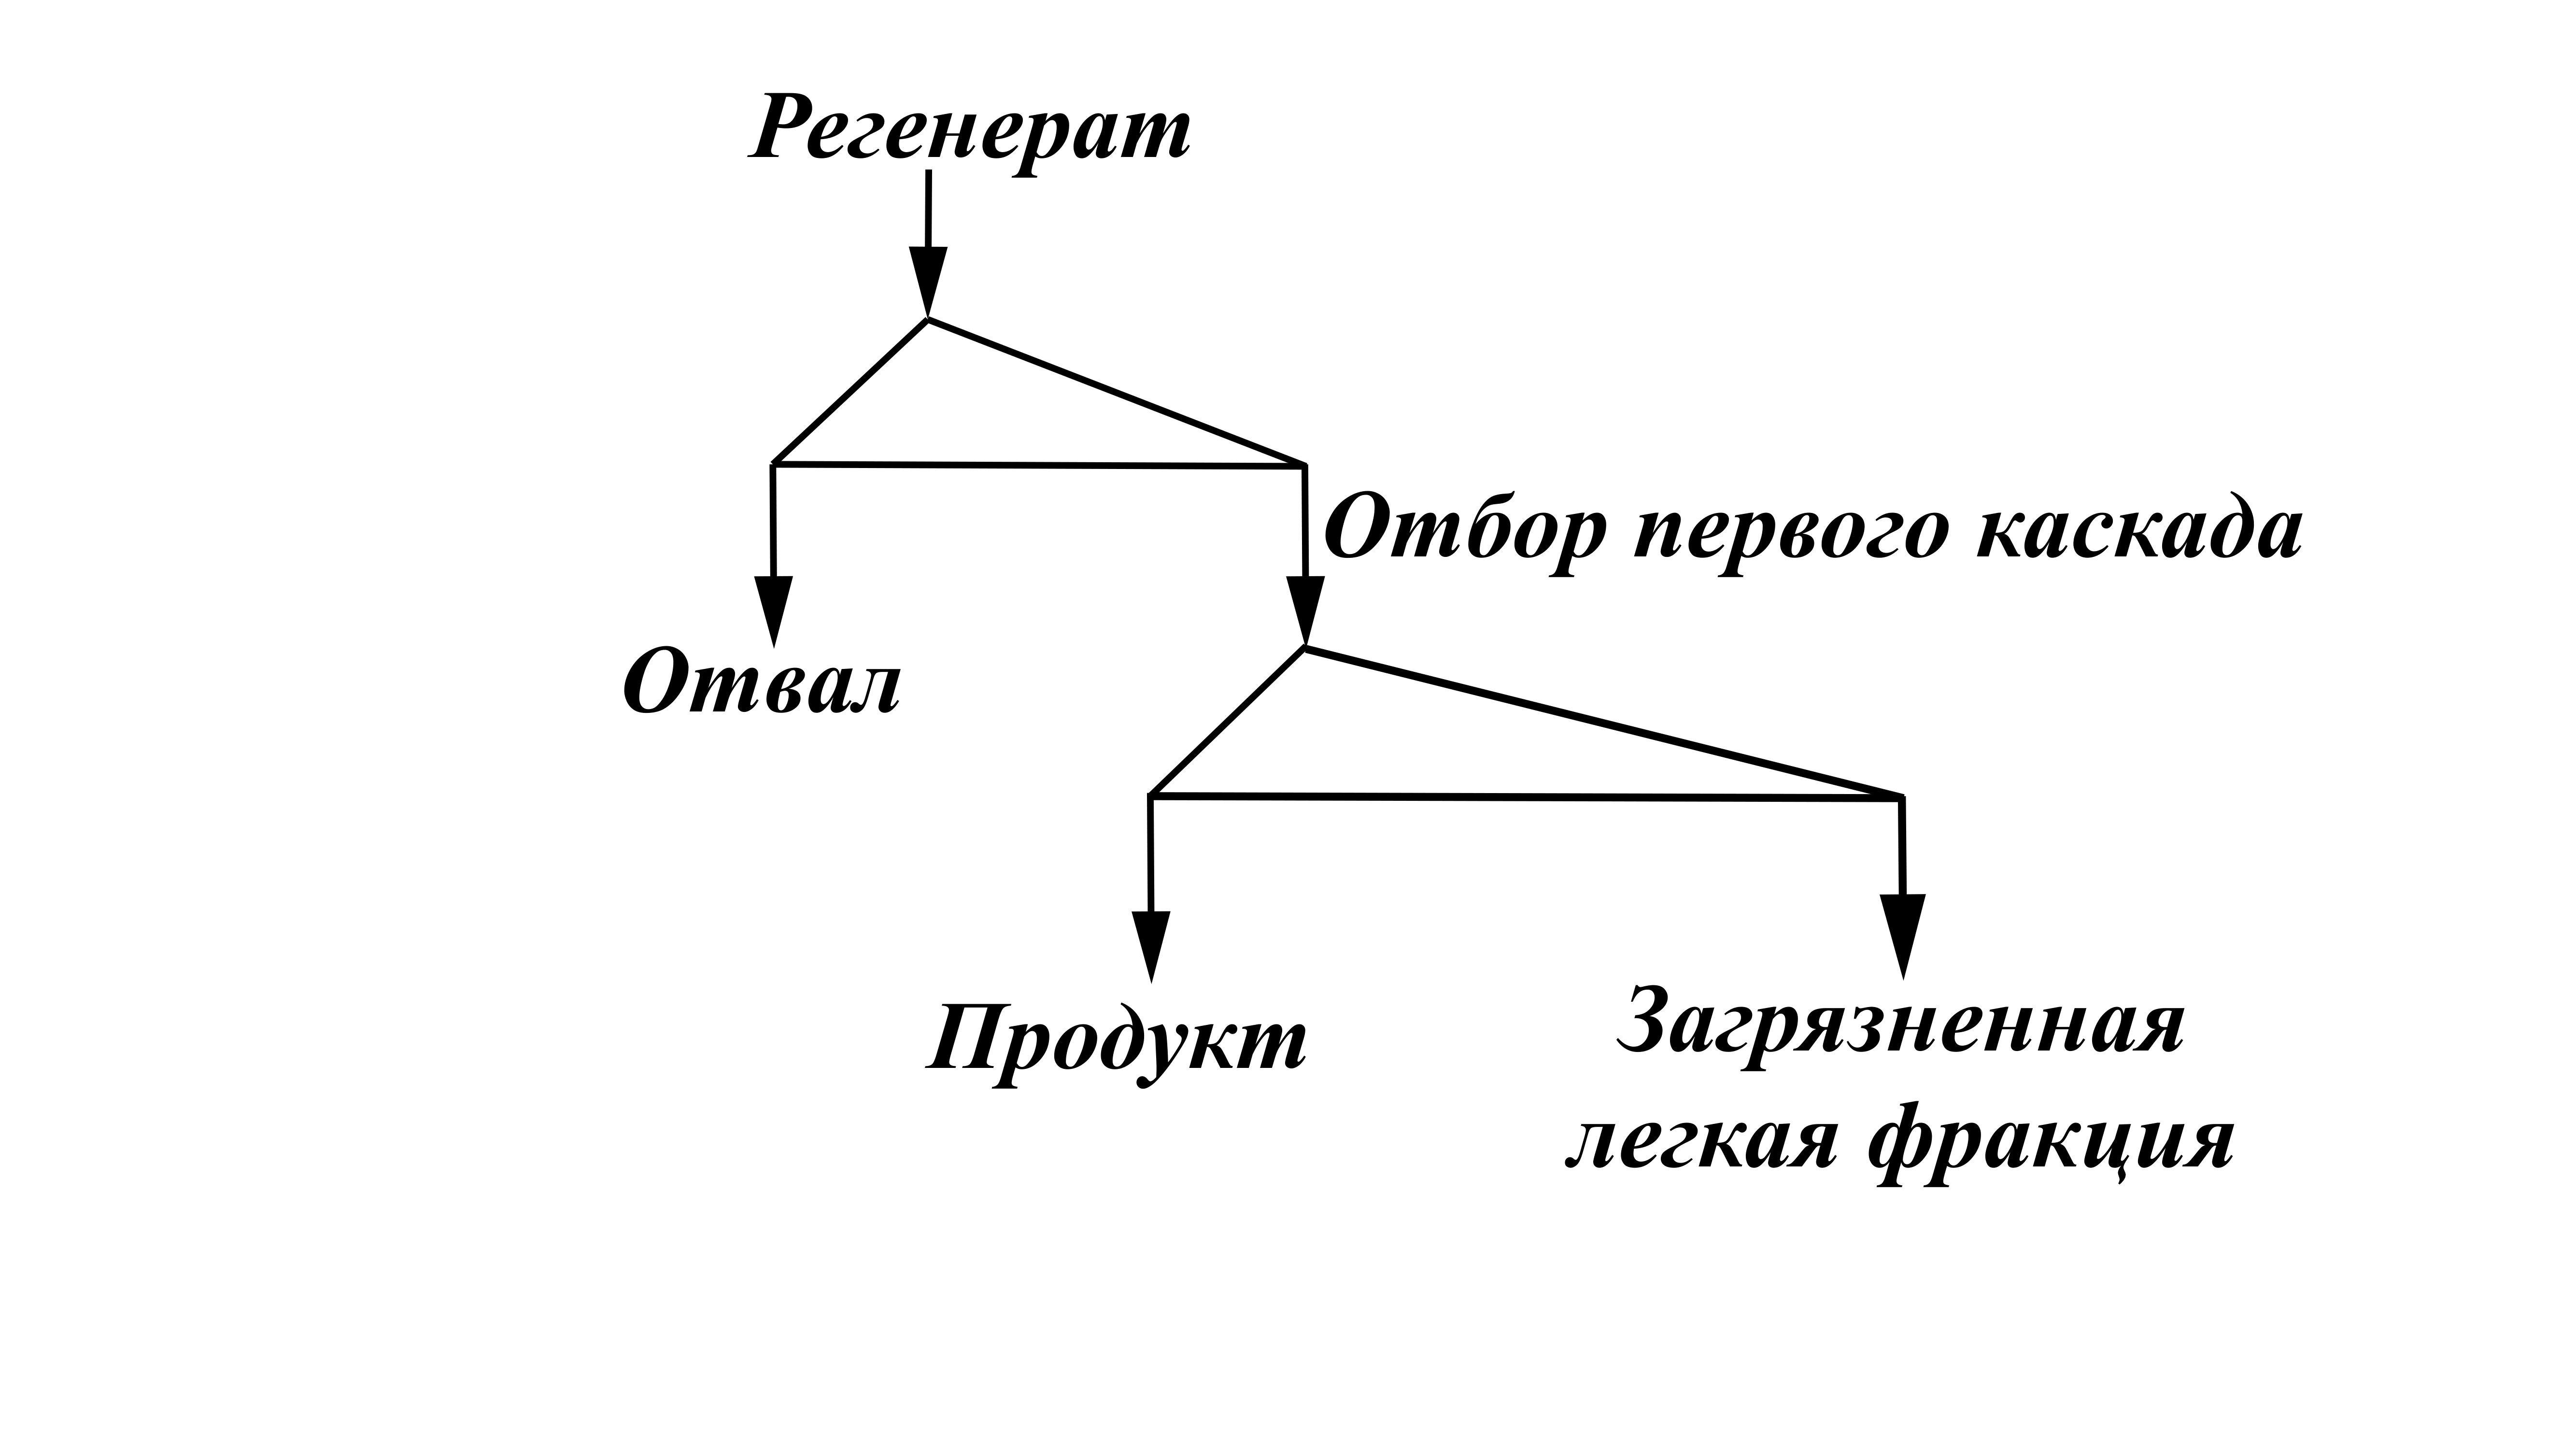
\includegraphics[scale=0.07]{cascades/double_ru}}
  \caption{Двойной каскад}\label{fig:double_ru}
\end{figure}

Физический эффект, который происходит в легком конце второго каскада, позволяющий сконцентрировать в нем четные изотопы $^{232,234}$U, чтобы уменьшить их выход в продукте, заключается в следующем. Когда концентрация $^{235}$U повышается до высокого уровня, соответствующего высокообогащенному урану (ВОУ) с $^{235}$U > 20\% или близкому к этому значению, наблюдается разворот монотонно возрастающей концентрации $^{235}$U, при том что прекращения роста концентрации $^{232,234}$U (а также $^{233}$U, который учитывается не во всех рассмотрениях) не происходит. Такая особенность массопереноса в каскаде обусловлена тем, что изотопы $^{232,234}$U обладают более высокими относительными коэффициентами обогащения, являясь самыми легкими в ряду изотопов урана \cite{borodynyaIssledovanieProblemyVovlecheniya1989}.  С помощью этого приема во втором каскаде и достигается <<пространственное>> разделение легкой фракции с изотопами $^{232,233,234,235,236}$U и тяжелой с $^{235,236,238}$U, в чем и состоит основной принцип двойного каскадирования.

Однако, возможность удалять из изотопной смеси легкие четные изотопы сопряжена с потерями ценного $^{235}$U в виде высокообогащенного урана в выводимом потоке. Кроме того, так как результирующая побочная смесь содержит повышенную долю $^{232,234}$U, это обстоятельство накладывает жесткие ограничения на обращения с таким радиотоксичным материалом, поэтому особенно остро встает вопрос об окончательной утилизации этого материала. Таким образом, загрязненность побочно произведенной фракции легкими изотопами, и, в особенности, изотопом $^{232}$U, требует особых условий обращения с ней, а окончательная утилизация может быть крайне дорогостоящей операцией \cite{smirnovApplyingEnrichmentCapacities2018}.

Эти два фактора, связанные с появлением в схеме легкой высокообогащенной фракции второго каскада, составляют основную проблему составных каскадов, как двойных (рис. \ref{fig:double_ru}), так и сконструированных на основе двойных, пути решения которой будут описаны в последующих разделах.

В качестве примера реализации схемы двойного каскада, в патенте \cite{vodolazskihSposobIzotopnogoVosstanovleniya} предлагается обогащать изотопную смесь регенерата до уровня оружейного (> 90\% $^{235}$U) уже в первом ординарном каскаде. Такой подход позволяет добиваться содержания $^{232}$U в тяжелой фракции второго каскада на уровне сырьевого регенерата.

Существуют также реализации, когда схема двойного каскада (рис. \ref{fig:double_ru}) подразумевает использование газа-носителя (или буферного газа) \cite{prusakovCorrectingIsotopicComposition2008, SposobIzotopnogoVosstanovleniyab}. Применяемое буферное газообразное соединение должно является инертным (неактивным) к гексафториду урана -- рабочему газу. Использование газа-носителя может позволить повысить эффективность отделения $^{232}$U от регенерированного урана и уменьшить потери $^{235}$U. Впервые идея применения такого газа с массовым числом, близким к $^{232}UF_6$, была выдвинута в \cite{SosninYuChelcov}, исходя из предположения, что такой газ мог бы служить матрицей-носителем для $^{232}UF_6$.
В этом исследовании авторы предложили использовать фреон-346 $C_{8}H_{3}F_{13}$, поскольку среднее массовое число этого соединения практически совпадает с массовым числом молекулы $^{232}UF_6$ (и ниже, чем у $^{235}UF_6$, что важно для предотвращения извлечения $^{235}$U в потоке газа-носителя). К тому же, $C_{8}H_{3}F_{13}$ является инертным по отношению к гексафториду урана и не вступает в реакцию с материалами газовой центрифуги. Однако такой подход накладывает ограничения на допустимый интервал давлений в разделительном процессе, который обусловлен центробежным полем газовой центрифуги \cite{prusakovCorrectingIsotopicComposition2008}.

Оба рассматриваемых варианта двойного каскада, как с газом-носителем, так и без, разделяют следующие недостатки:
\begin{enumerate}
  \item оба каскада в схеме загрязнены изотопом $^{232}$U, что осложняет радиационную обстановку на разделительном производстве.
  \item в предлагаемой схеме принципиально отсутствует возможность снижения накопления изотопа $^{236}$U, негативное влияние которого на размножающие характеристики тепловыделяющих сборок (ТВС) требует дополнительного обогащения по изотопу $^{235}$U. При этом эквивалентная концентрация $^{235}$U может быть заметно больше, чем в штатном топливе, что обуславливает дополнительные затраты работы разделения.
\end{enumerate}

При этом вариант с газом-носителем, требует очистки получаемого товарного продукта от этого газа, что, очевидно, также приводит к увеличению удельных затрат. Отсюда, вариант без несущего газа более предпочтителен, поскольку в ходе технологических операций не возникает необходимости очищать от него выходную смесь \cite{smirnovKaskadnyeShemyZadachah2012}.

Среди недостатков двойного каскада следует отметить, что некоторые его реализации предполагают получение высокообогащенного урана с содержанием $^{235}$U более 20\%, что усложняет проблему соответствия международным стандартам обращения с делящимися материалами.
Так, в \cite{palkinPurificationReprocessedUranium2016} подчеркивается, что, тогда как уже в первом же каскаде достигается концентрация $^{235}$U >20\%, которая затем во втором каскаде еще больше повышается в потоке легкой фракции, такая схема может быть неприемлема ввиду строгих ограничений на производство ВОУ во всем мире \cite{ManagementHighEnriched2005}.

Для решения проблемы возникновения ВОУ, предложен вариант реализации двойного каскада, в котором исключаются высокие концентрации $^{235}$U \cite{zhurinSposobIzotopnogoVosstanovleniya2010}. В таком исполнении, принцип работы несколько меняется (рис. \ref{fig:pure_double}).
В этом каскаде очистка от четных изотопов $^{234,234}$U производится в первом ординарном каскаде с последующим выведением потока легкой фракции из системы. Затем, целевой продукт, восстановленный по изотопному составу, нарабатывают в легкой фракции второго каскада. Такой подход позволяет <<отсекать>> от смеси изотопы $^{234,234}$U уже в первом ординарном каскаде, передавая на второй смесь, содержащую, в основном, изотопы $^{235,236,238}$U \cite{borodynyaIssledovanieProblemyVovlecheniya1989}. А делящийся изотоп $^{235}$U, имея относительный коэффициент обогащения (относительно $^{238}$U ) вышем, чем $^{236}$U, во втором каскаде будет концентрироваться в легком конце с более высокой скоростью.

\begin{figure}[ht]
  \centerfloat{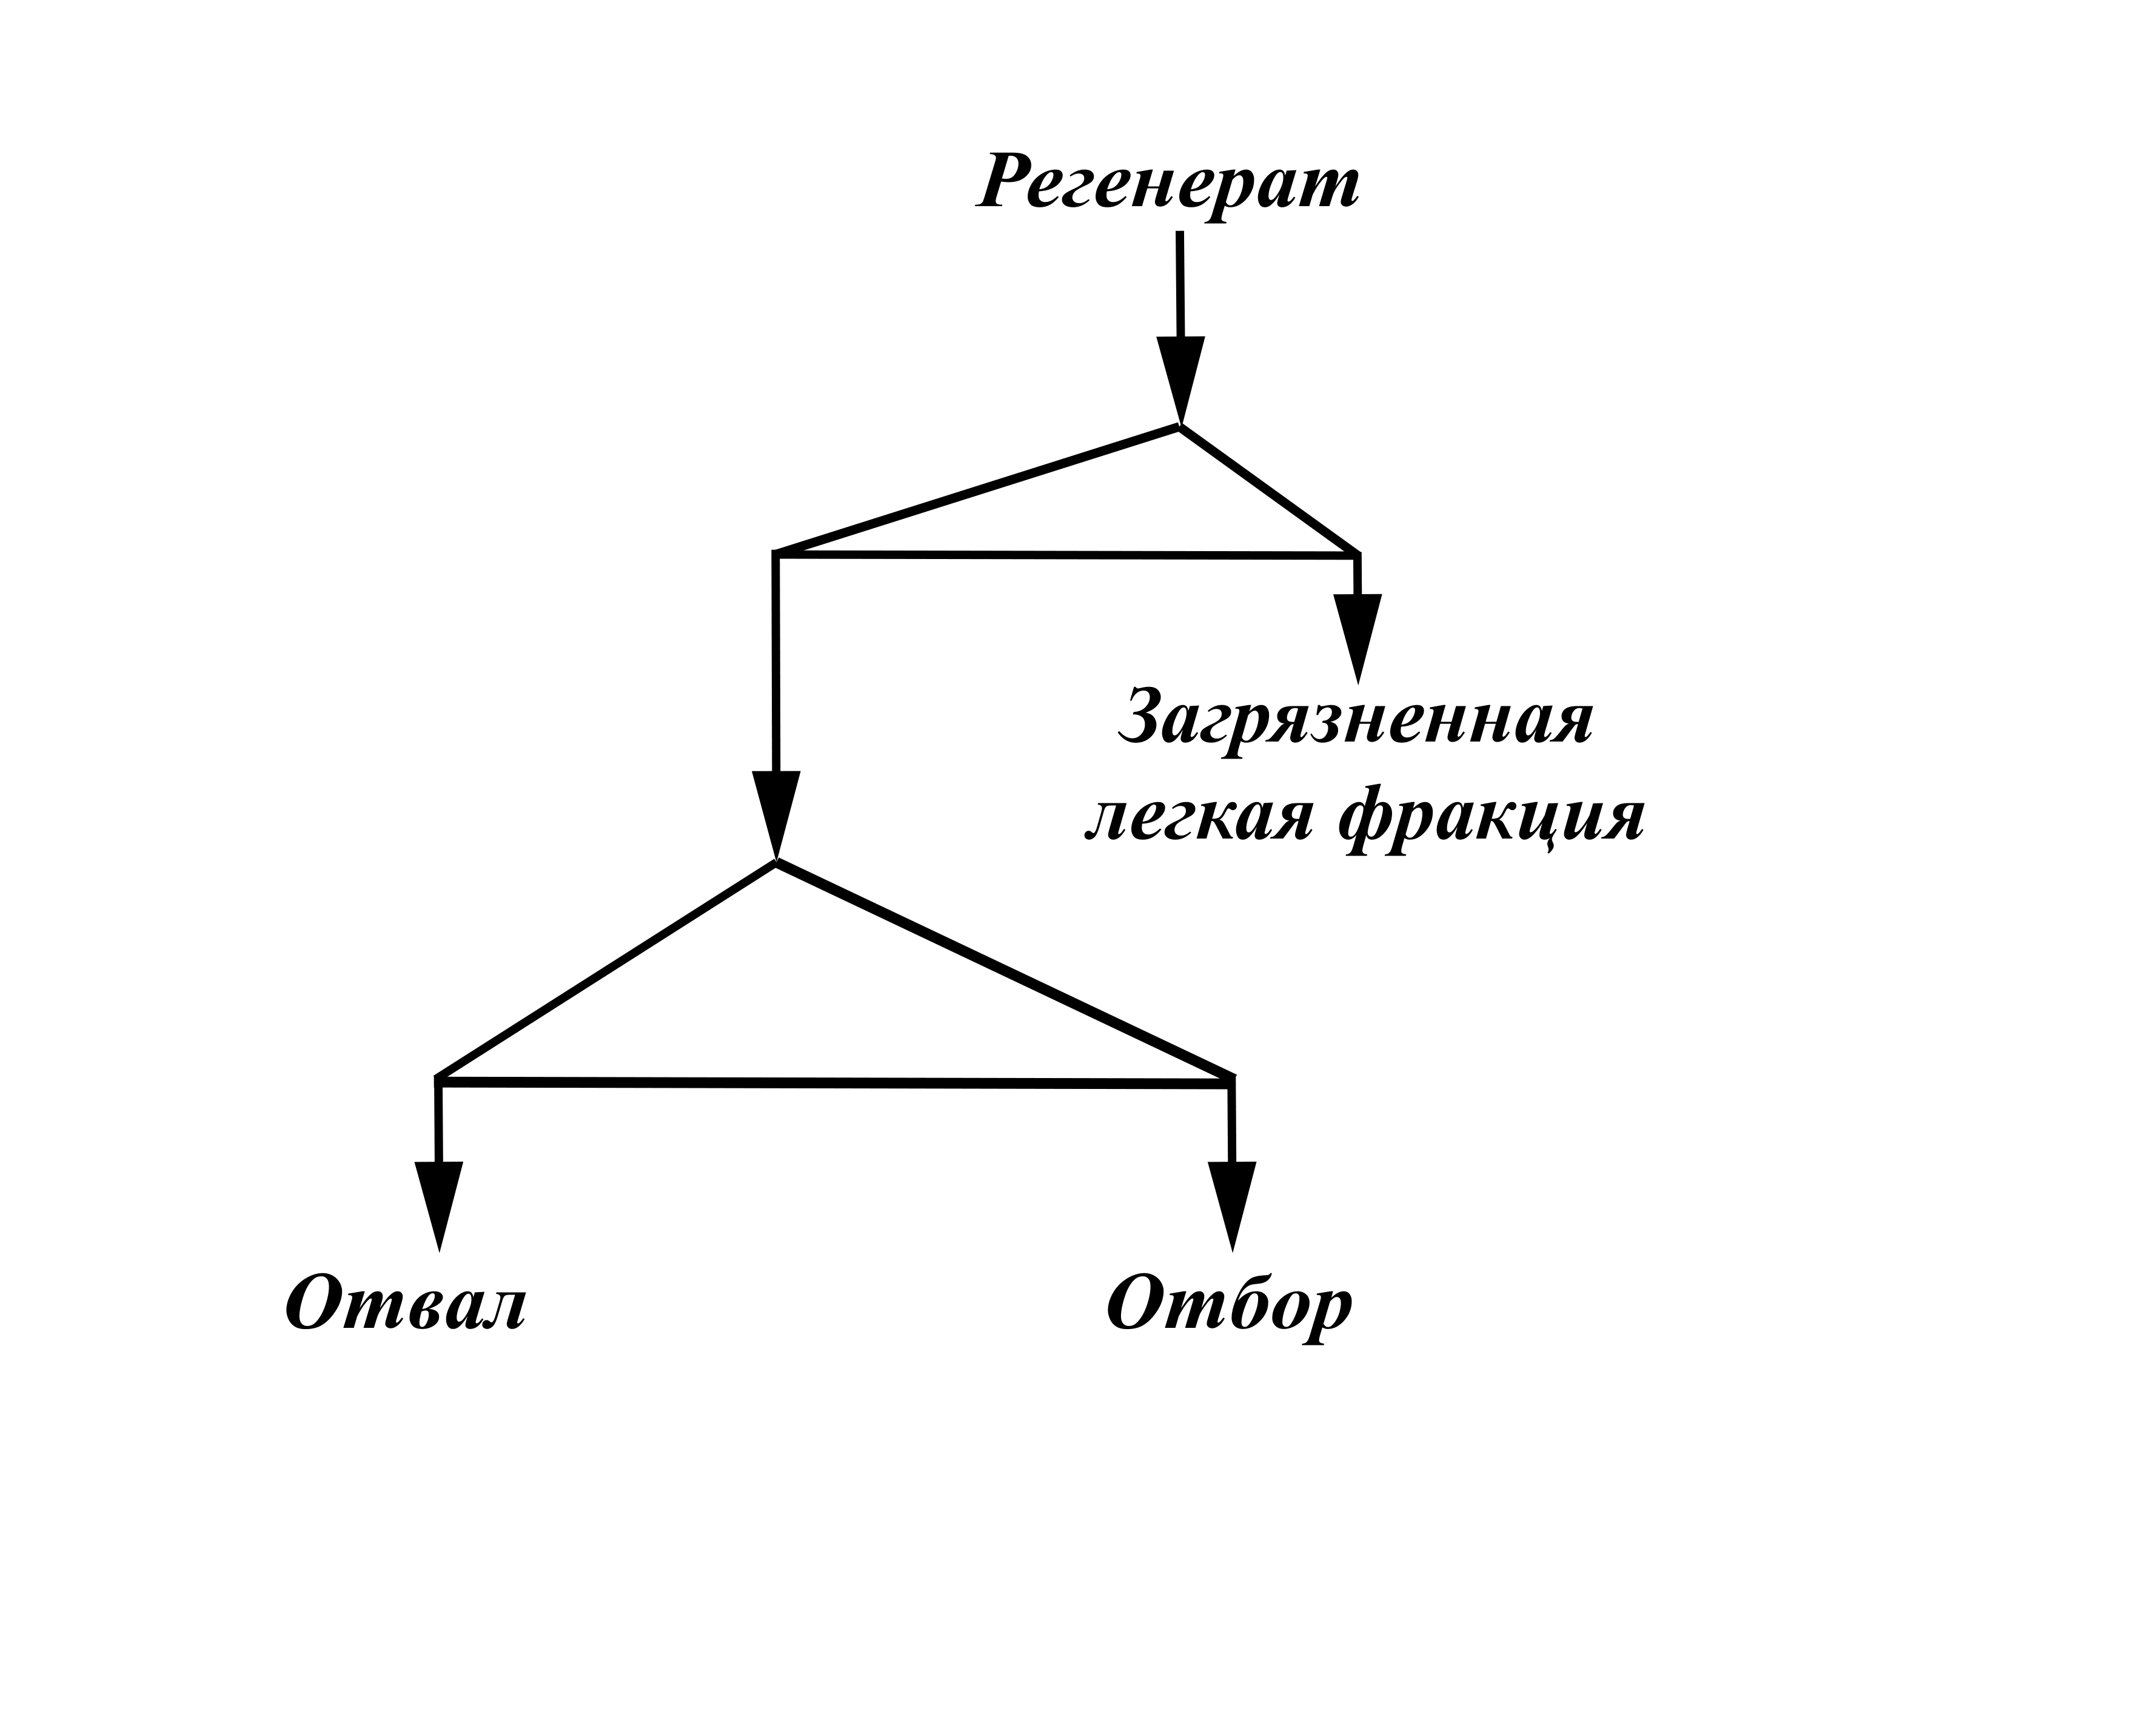
\includegraphics[scale=0.1]{cascades/pure_double}}
  \caption{Двойной каскад с очисткой в первом каскаде}\label{fig:pure_double}
\end{figure}


Здесь второй каскад запитывается тяжелой фракцией первого каскада, полученной при обогащении легкой фракции первого каскада изотопом $^{235}$U до концентрации,не превышающей 20\%. В такой варианте схемы двойного каскада роль каскада, на котором производится очистка от легких четных изотопов, принимает первый ординарный каскад.

Как частный случай такой схемы в работе \cite{palkinReprocessedUraniumPurification2013} предлагают использовать прием смещения точки подачи питания в сторону точки отбора легкой фракции первого каскада, так как это позволяет добиться существенного снижения доли $^{232}$U в конечном продукте, так как прохождение самым легким изотопом меньшего количества последовательных ступеней каскада позволяет <<отложить>> достижение им пиковой концентрации к отборной ступени легкой фракции. а также, Высокая же степень обогащения в первом каскаде или, иными словами, длинная обогатительная часть каскада, позволяет добиться концентрирования большей доли $^{234,236}$U в выводимом из системы потоке, что ведет к более низкому содержанию этих изотопов в конечном продукте. Однако, такой вариант связан с существенными потерями работы разделения, которые возникают при смешении в ступенях каскада потоков с различными концентрациями целевого компонента $^{235}$U, и не позволяет осуществлять достаточно эффективную очистку от $^{234,236}$U \cite{palkinPurificationReprocessedUranium2016}.

% В главе 3 будет приведен расчетный анализ для выявления физических закономерностей, позволяющих судить о пригодности таких схем для задачи обогащения регенерата в условиях многократного рецикла.

Итак, двойной каскад имеет уникальное преимущество, которое состоит в возможности повторно обогащать регенерированный уран, не разбавляя его дополнительным сырьем, в качестве которого, как правило, используется природный уран или его производные. Это свойство обуславливает предпочтительность двойного каскада с точки зрения экономии природного урана. Однако оно не предотвращает потерь $^{235}$U из топливного цикла в удаляемом потоке легкой фракции, используемой с целью вывода из системы нежелательных изотопов легкой группы $^{232,234}$U. Также схема двойного каскада не может обеспечить условие полного возврата -- возврата эквивалентного производимому продукту количества облученного материала в ядерный топливный цикл топлива в цикл -- в условиях многократного использования топлива \cite{smirnovObogashchenieRegenerirovannogoUrana2018}. Это означает, что для загрузки реактора, в котором используется переработанное топливо, необходимо будет использовать другой источник делящегося изотопа $^{235}$U, например, природный уран, в отдельных тепловыделяющих элементах (ТВЭЛах) или целых ТВС. В результате, в контексте замыкания ЯТЦ по урановой составляющей и возврата в топливный цикл реактора всего объема топлива, реальная экономия природного урана будет не 100\%, а в несколько раз меньше -- в лучшем случае 15-20\%.

Чтобы решить проблему невозможности полного возврата регенерата, добившись желаемого соотношения финального продукта и питающего регенерата, потребовалась модификация схемы двойного каскада, предложенная в работе \cite{smirnovObogashchenieRegenerirovannogoUrana2018} в рамках диссертационного исследования. Она будет рассмотрена в основной части диссертационной работы (глава \ref{ch:ch3}).
% Далее продолжим детальное рассмотрение иных возможных комбинаций каскадов.

\subsubsection{Составные каскадные схемы}
Рассмотрим другие способы коммутации каскадов в составные схемы.

В работе \cite{OChISTKAREGENERIROVANNOGOURANA2013} (или указать оригинал \cite{palkinReprocessedUraniumPurification2013}?) предложена схема, представленная на рис. \ref{fig:double_palk}. Принцип ее работы состоит в следующем.

\begin{figure}[ht]
  \centerfloat{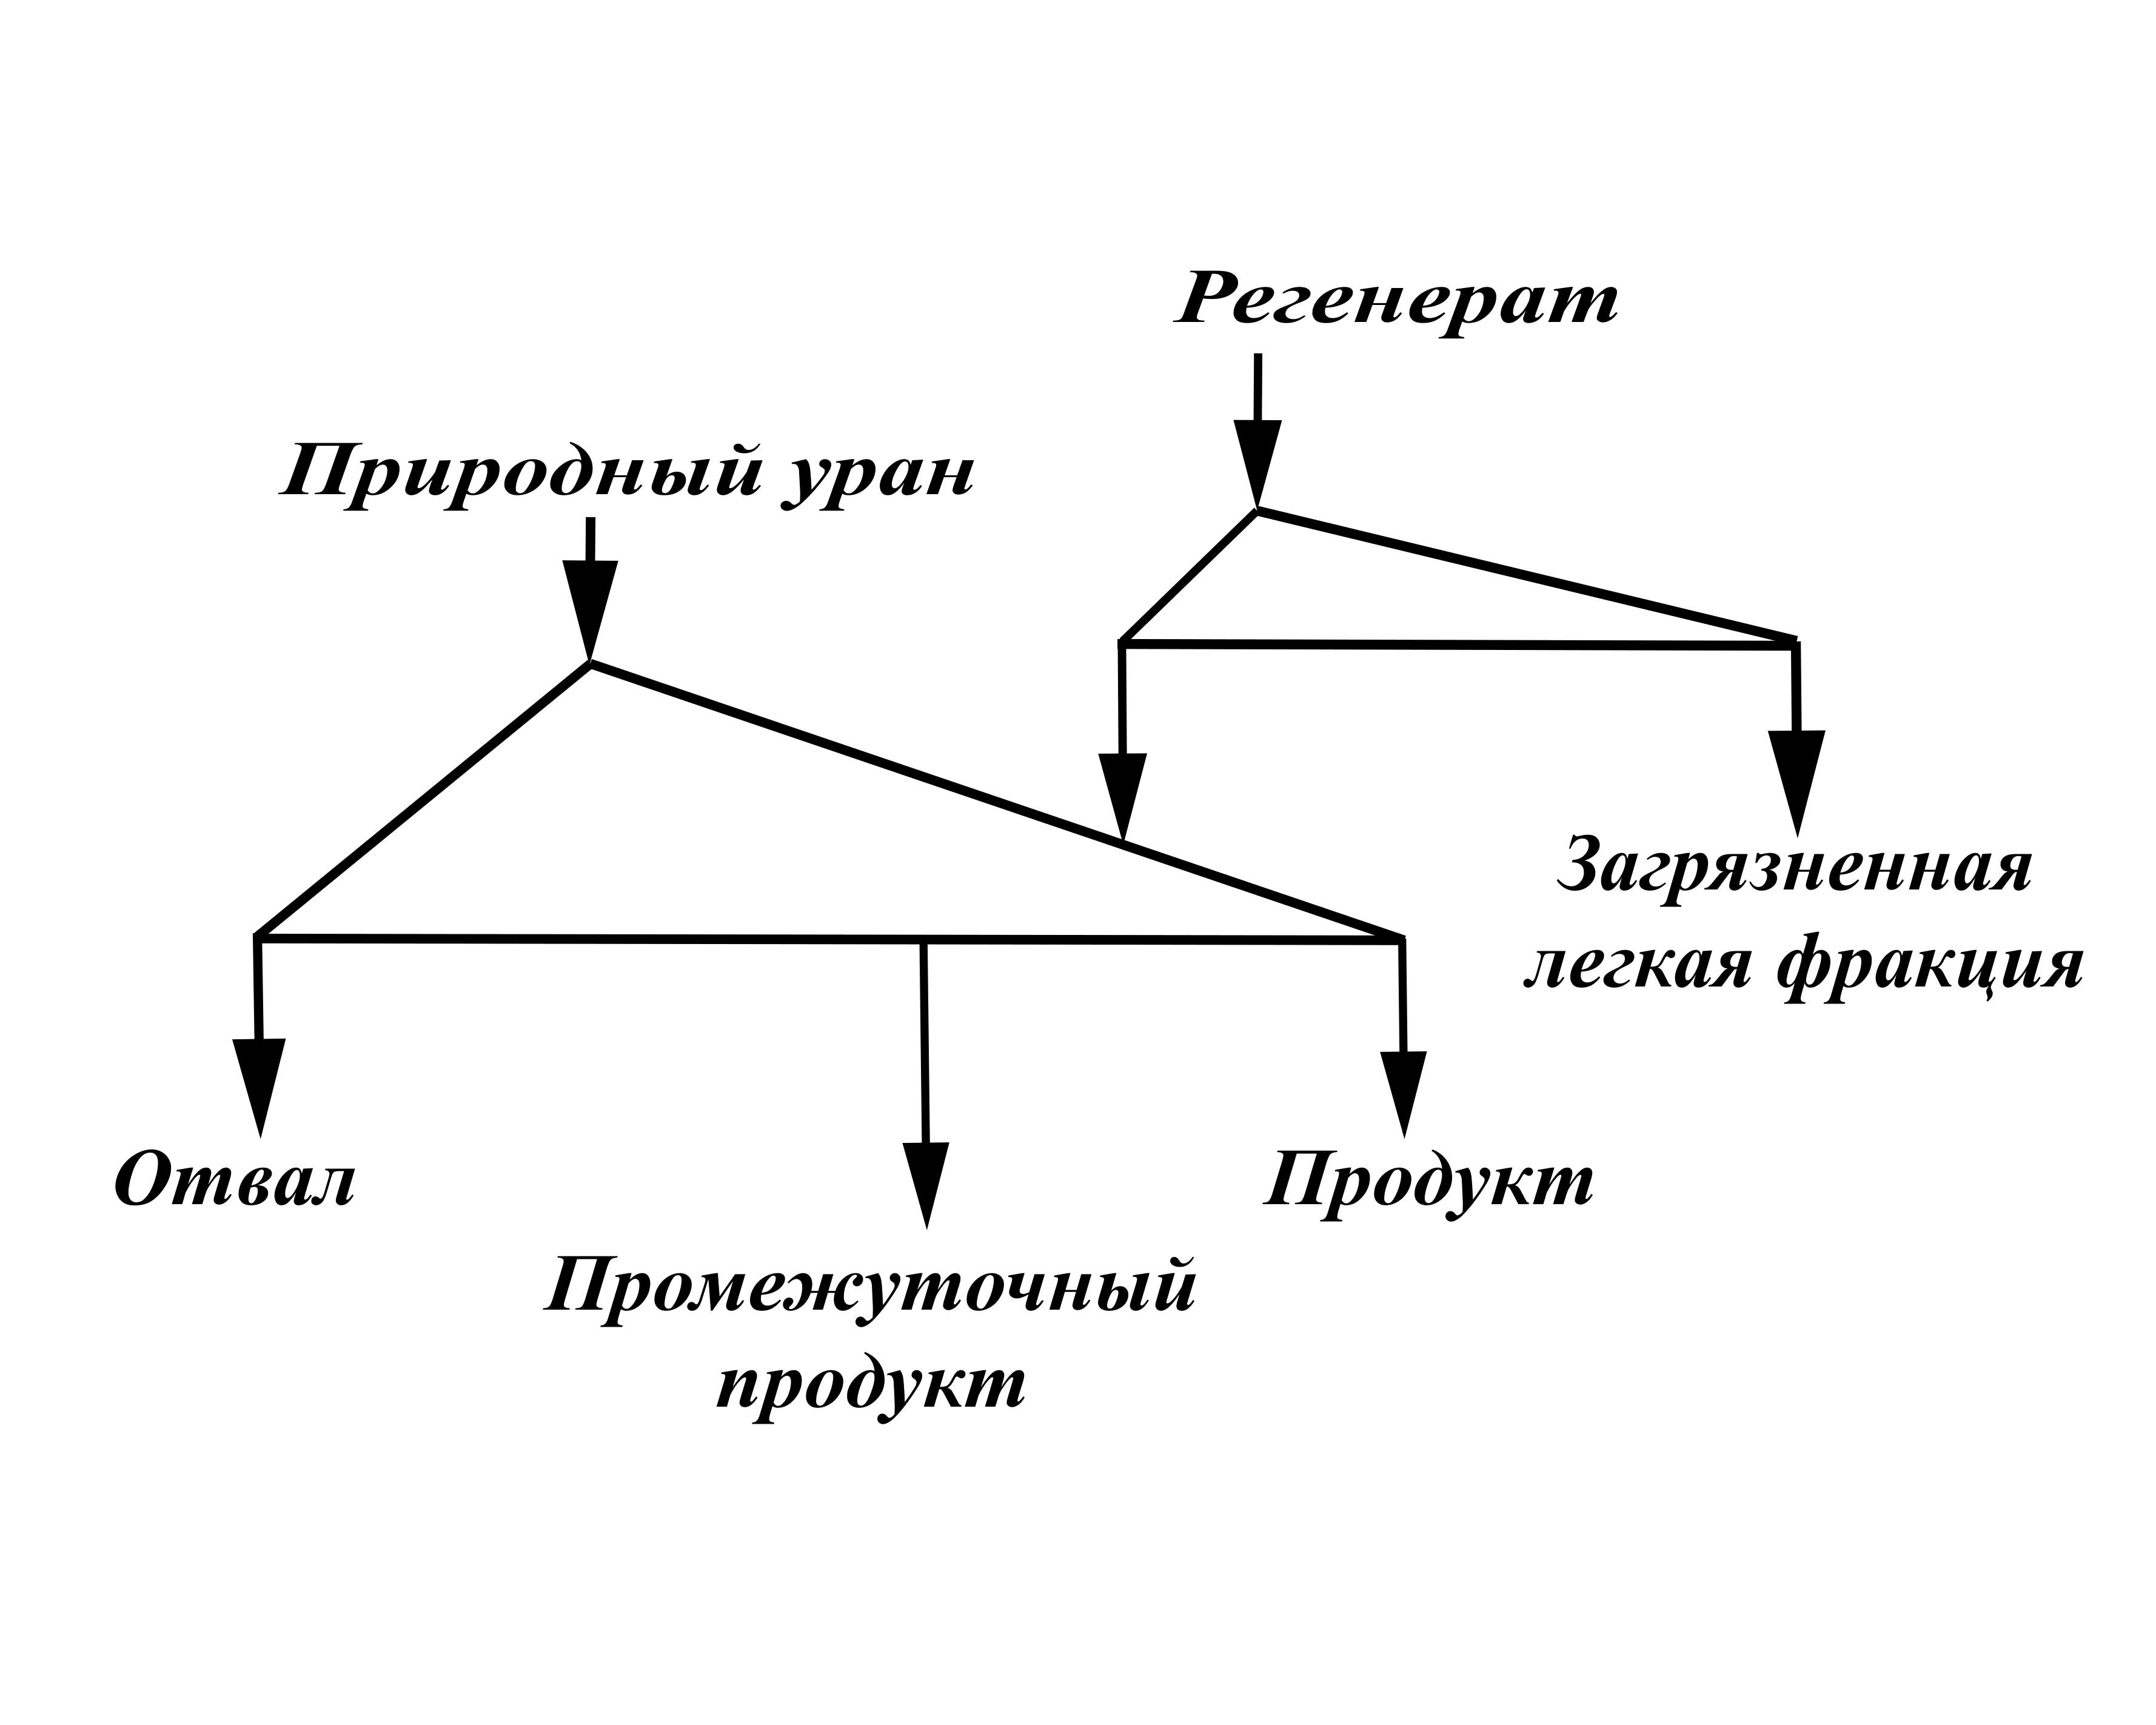
\includegraphics[scale=0.1]{cascades/double_palk}}
  \caption{Двойной каскад, использующий две стадии очистки}\label{fig:double_palk}
\end{figure}


Первый каскад, питаемый регенератом, концентрирует изотопы $^{232}$U и $^{234}$U на легком конце как в схеме двойного каскада с очисткой в первом каскаде (рис. \ref{fig:pure_double}). Полученная на другом конце смесь тяжелой фракции первого каскада подается на промежуточную ступень второго каскада, питаемого природным ураном. Точка подачи питания этого дополнительного потока на основе очищенного регенерата подбирается по такому же принципу как и в уже рассмотренной схеме с дополнительным питанием (рис. \ref{fig:3_out}), чтобы избежать смешения потоков с различным содержанием $^{235}$U и связанных с этим потерь работы разделения. Одиночный каскад в этой схеме, питаемый природным ураном, принципиально соответствует схеме каскада с двумя питаниями и дополнительным отбором (рис. \ref{fig:3_out}), с тем отличием, что регенерированный питающий уран проходит дополнительную предварительную стадию очистки в ординарном каскаде перед поступлением в последующий каскад в качестве дополнительного питания. В результате, такая схема позволяет частично выводить из системы нежелательные четные изотопы $^{232,234}$U, оставаясь в рамках заданных ограничений, производя на выходе НОУ-продукт товарного качества и дополнительное количество промежуточного продукта с пониженным содержанием $^{232,234}$U, относительно исходного регенерата. Вдобавок, такая схема позволяет соблюсти ограничения на получение высокообогащенного урана, не предполагая выхода за 20\% по  $^{235}$U.
Дальнейшего усовершенствования схемы можно достичь с помощью оптимизации концентрации $^{232}$U в продукте, варьируя точку подачи, при этом минимизируя количество газовых центрифуг, аналогично приему, описанному для схемы двойного каскада с очисткой регенерата в первом каскаде (рис. \ref{fig:pure_double}). В этом случае, в отвальном конце каскада будет на порядок снижено содержание вредного $^{232}$U.
Эта стадия позволяет подготовить из регенерированного урана изотопный состав с меньшим содержанием $^{232}$U для последующих этапов обогащения.

Однако, будучи модификацией схемы каскада с двумя питаниями, одним отвалом, основным и дополнительным отбором, такая конфигурация наследует и его недостаток, заключающийся в том, что высокое качество очищенного регенерата достигается только при малой доле потока питающего регенерата относительно природного урана. Иными словами, ввиду малости потока регенерата относительно потока природного урана, такая схема может квалифицироваться скорее как схема разбавления регенерата природным, чем очищающая его от $^{232,234}$U. Ввиду этого, она не позволяет достичь полного возврата регенерата в цикл в условиях многократного использования ядерного топлива.


Существует еще одна модификация двойного каскада, использующая в качестве одного из составных элементов каскад с двумя питаниями, одним отвалом, основным и дополнительным отбором. Такая схема предложена в патенте \cite{SposobIzotopnogoVosstanovleniyac} (рис. \ref{fig:double_crazy}). Принцип ее работы состоит в следующем.

\begin{figure}[ht]
  \centerfloat{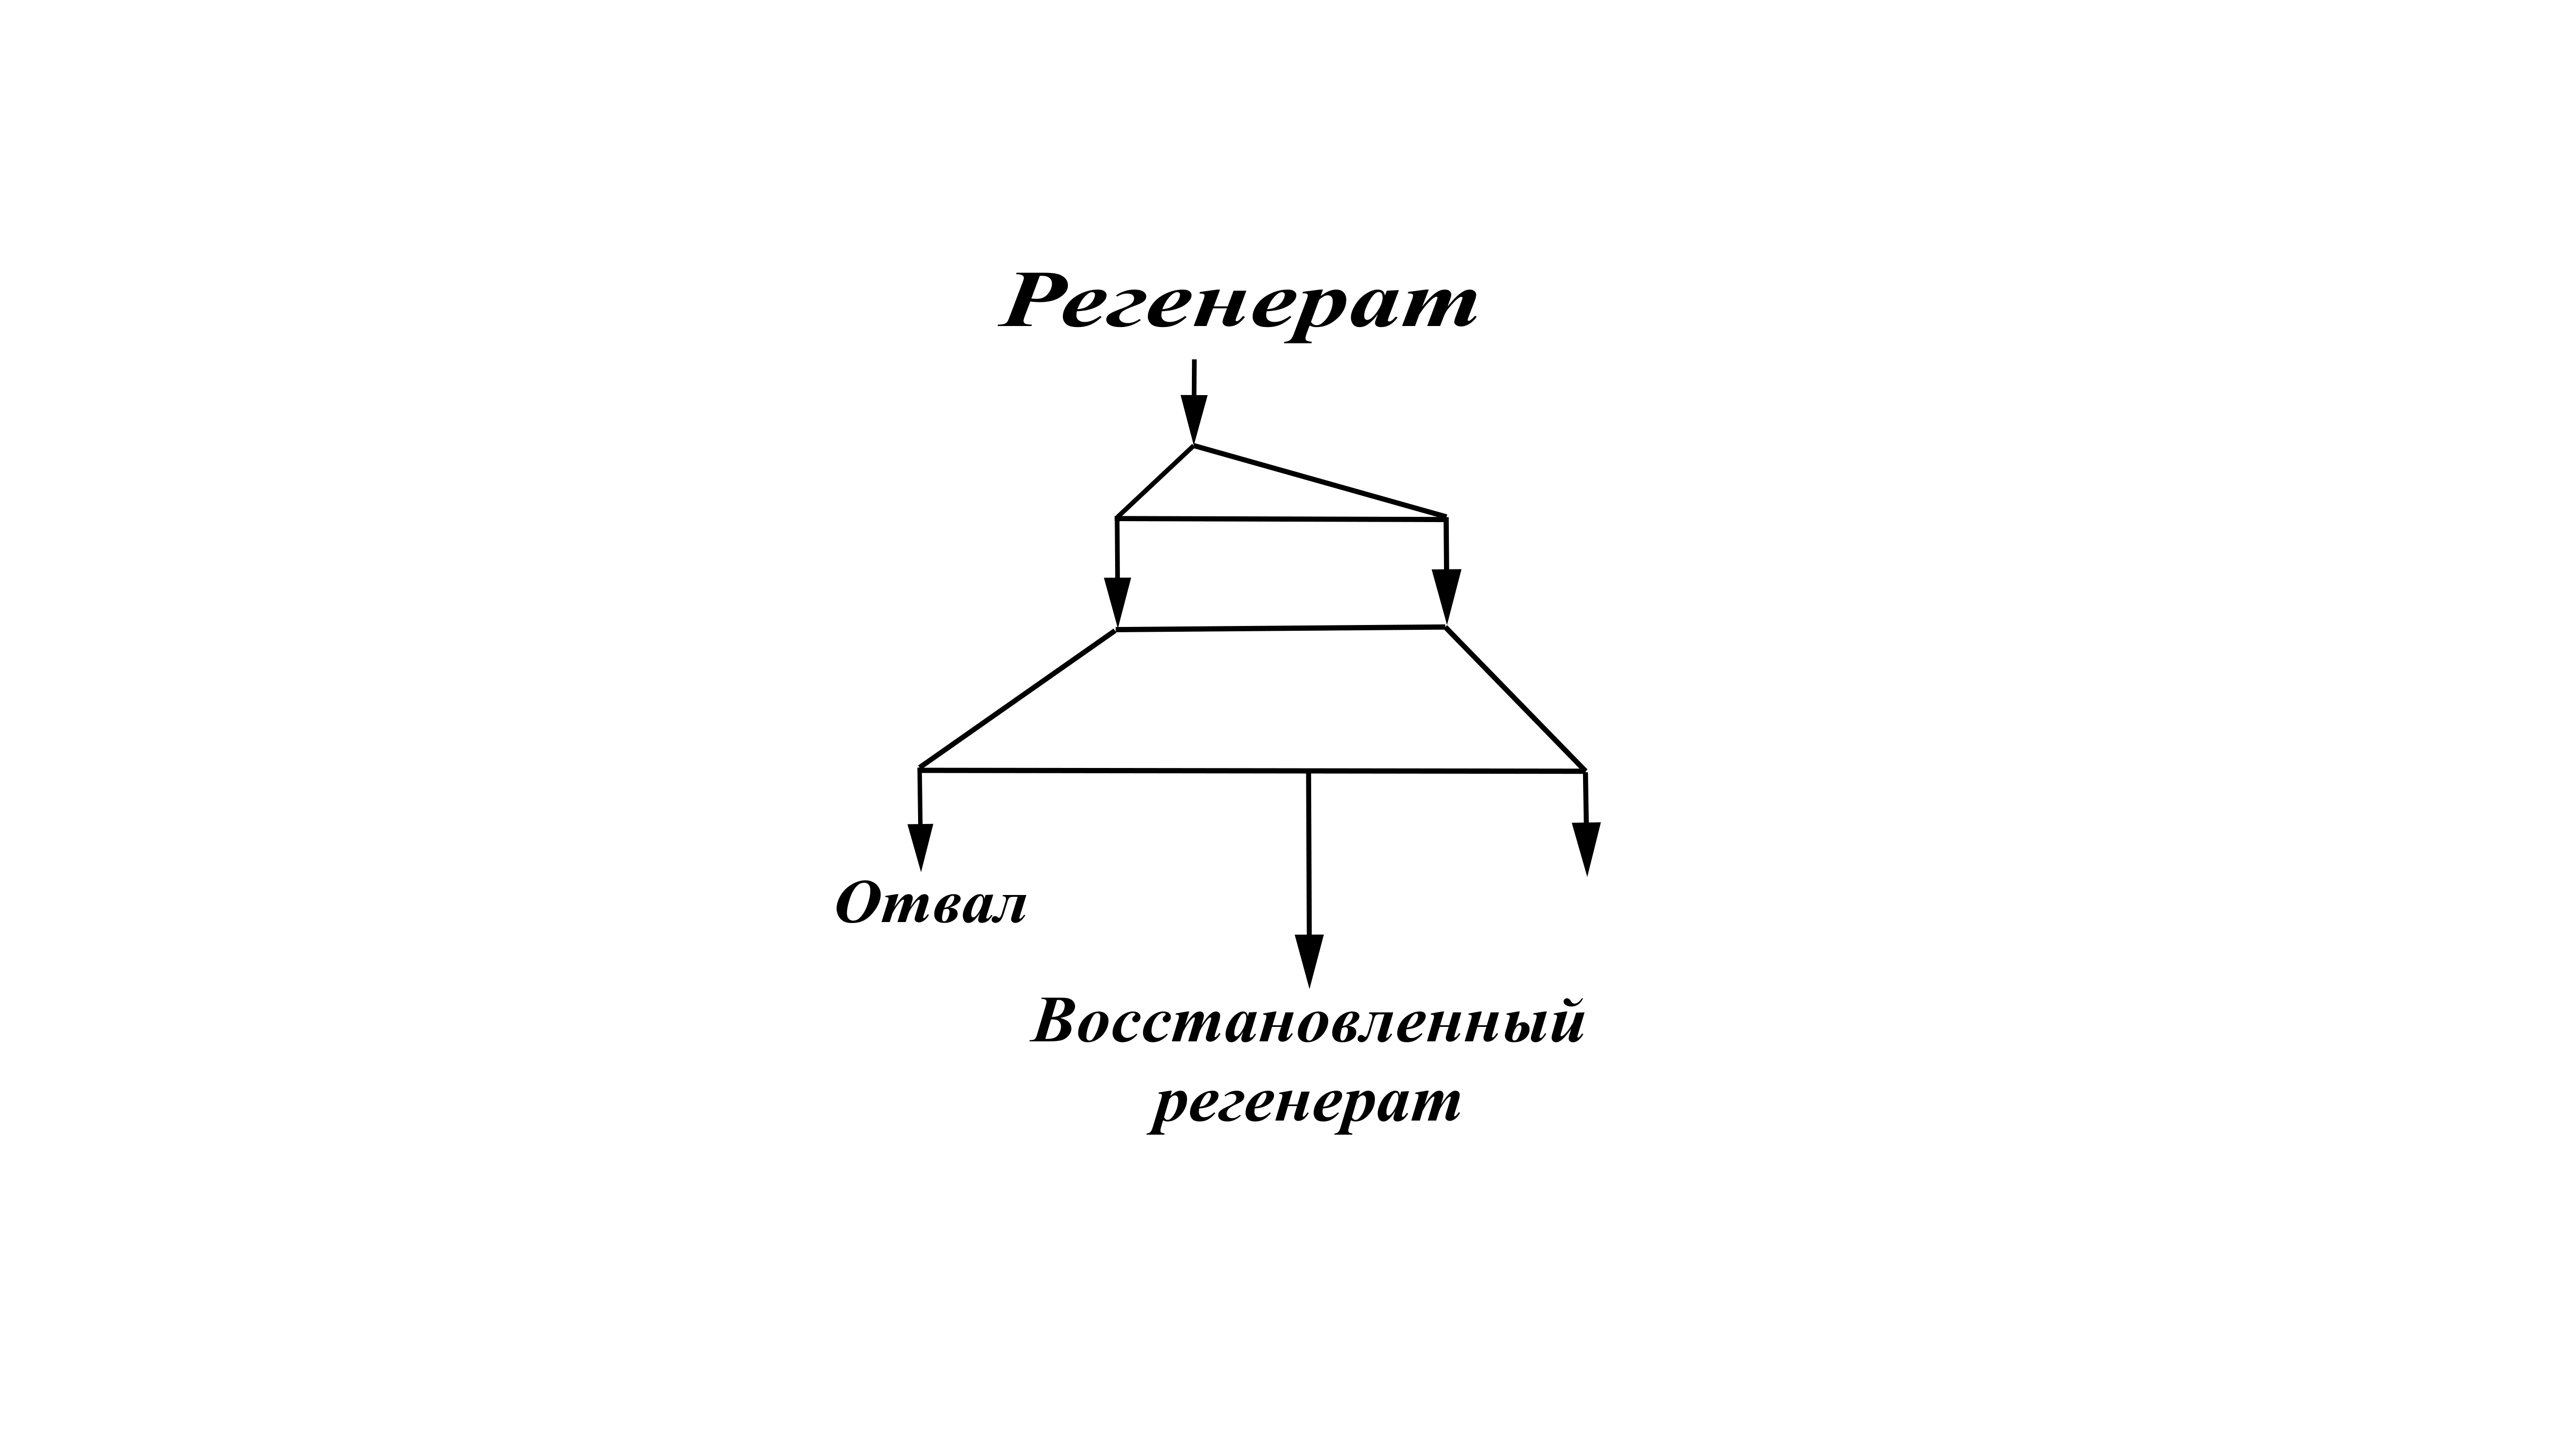
\includegraphics[scale=0.1]{cascades/double_crazy}}
  \caption{Двойной каскад, производящий восстановленный регенерат в промежуточном потоке отбора}\label{fig:double_crazy}
\end{figure}

Первый каскад (верхний на рис. \ref{fig:double_crazy}) обогащает регенерированный уран до $5,0-10,0$\% по $^{235}$U, а потоки отвала и отбора направляются на питание второго каскада. Во втором каскаде в потоке дополнительного отбора производится изотопно-восстановленный регенерированный уран с пониженной концентрацией $^{232,234}$U. Этот промежуточный продукт пригодный для прямого использования в производстве НОУ (с помощью обогащения в ординарном трехпоточном каскаде), как было показано в разборе схемы с дополнительным отбором, извлекается из промежуточной ступени второго каскада. Заявленной задачей изобретения является более полная очистка регенерата от $^{232}$U, достигаемая без необходимости использовать регенерированный уран. То есть данная схема предлагает очевидное преимущество в виде отказа от операции разбавления скорректированного изотопного состава регенерированного урана ураном природного происхождения. Однако, возможность извлечения $^{232}$U в такой схеме сильна ограничена.

Следует обратить особое внимание, что поток, произведенный в обогащающем (<<легком>>) конце второго каскада, имеющий категорию ВОУ, не находит свое применение. Этот изотопный состав смешивается с отвалом второго каскада, который позволяет экранировать гамма-излучение, обусловленное $^{232}$U. Такое решение минимизирует риски долговременного хранения невостребованных продуктов изотопной корректировки регенерированного урана.
То есть, это решение может быть использовано для устранения проблемы с потоком легкой фракции второго каскада схемы (рис. \ref{fig:double_ru}).

Продолжая обзор составных каскадных схем, рассмотрим схему двойного каскада, предложенную в \cite{smirnovDilutionRecycledUranium2015}, использующую каскад с тремя питаниями (рис. \ref{fig:double_3feeds}). Принцип ее работы состоит в следующем.

\begin{figure}[ht]
  \centerfloat{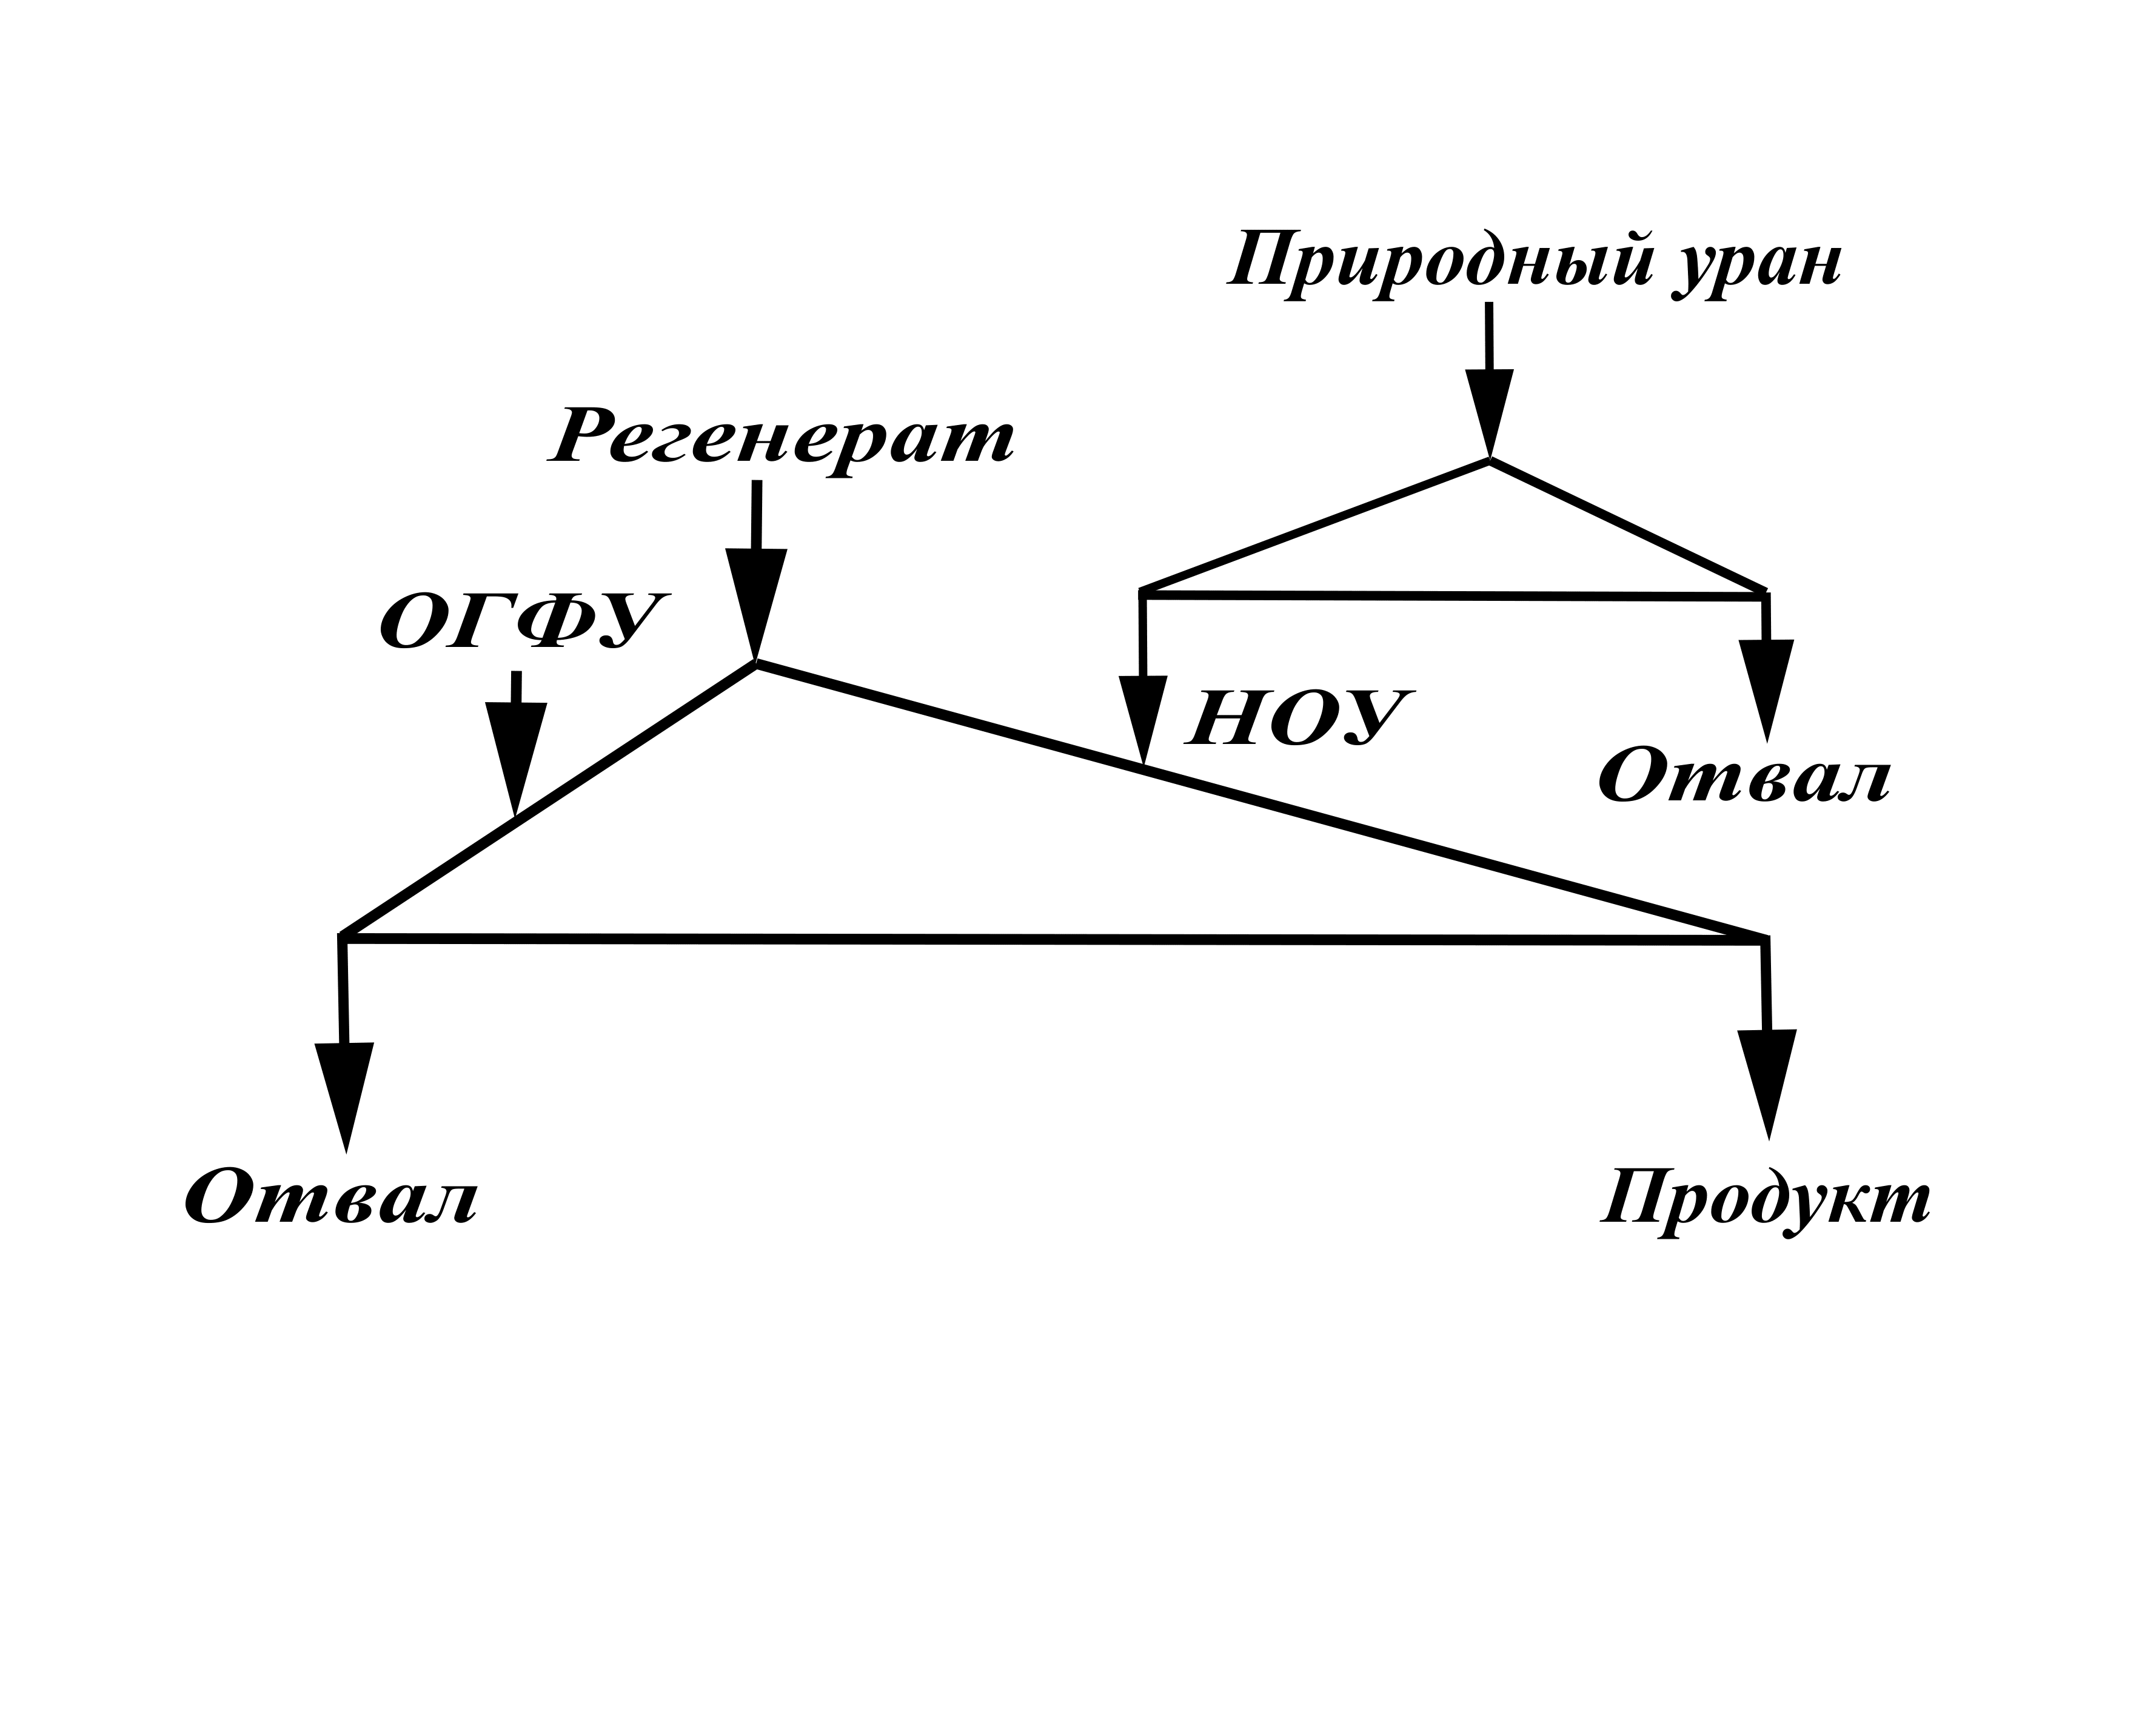
\includegraphics[scale=0.1]{cascades/double_3feeds}}
  \caption{Двойной каскад, использующий каскад с тремя питаниями}\label{fig:double_3feeds}
\end{figure}

Использование в качестве дополнительного потока питания каскада с тремя питаниями потока НОУ, вместо потока природного урана, позволяет достичь лучших показателей экономии природного урана и затрат работы разделения за счет обеспечение большего совокупного содержания изотопа $^{235}$U в каскаде с тремя питаниями. Эта схема получила дальнейшее развитие в \cite{smirnovEvaluatingEffectivenessDilution2016}, где было продемонстрирована возможность снизить с помощью нее себестоимость производства товарного НОУ-продукта. Однако, схемы на основе каскада с тремя питаниями (с двумя дополнительными потоками питания) не позволяют добиться выполнения условий полного возврата регенерата в цикл и, как и ранее рассмотренные схемы с дополнительными потоками питания, обеспечивают возможность вовлечения регенерата в топливный цикл преимущественно за счет его разбавления смесями, не содержащими $^{232}$U \cite{smirnovApplyingEnrichmentCapacities2018}.

\section{Обобщенный анализ рассмотренных схем}

Подводя итог раздела, известные на сегодняшний день технические решения основаны на:
\begin{enumerate}
  \item разбавлении регенерированного урана материалами, не содержащими минорных компонентов (например, природным ураном), на входе в разделительный каскад, на выходе из разделительного каскада или внутри каскада при наличии в нем двух питающих потоков (регенерат и разбавитель);
  \item получении регенерата с пониженным содержанием минорных изотопов в каскаде с двумя питаниями и двумя потоками продукта (отбора);
  \item выделении из смесей регенерированного урана изотопа $^{232}$U при помощи газа-носителя, или не используя газ-носитель, в последовательном соединении двух разделительных каскадов.
\end{enumerate}


Возможности и недостатки рассмотренных схем:
\begin{itemize}
  \item основная проблема схем первого типа на основе ординарного каскада состоит в наличии в таких схемах лишь одного выходящего потока, в котором, очевидно, будут одновременно концентрироваться как целевой изотоп $^{235}$U, так и нежелательные четные изотопы. Как следствие, такого вида схемы подходят лишь для обогащения относительно незагрязненных составов регенерата, в которых исходные содержания четных изотопов меньше (на порядок или более), чем их допустимые пределы. Это означает невозможность ее применения в условиях многократного рецикла.
  \item первые два типа схем основаны, преимущественно, на принципе разбавления изотопной смеси регенерата урана составами в которых отсутствуют изотопы $^{232,236}$U и отсутствует накапливающееся в ходе ядерных превращений дополнительное количество $^{234}$U, то есть смесями на основе природного урана. Отсутствие в них эффекта <<пространственного>> разделения изотопов легкой $^{232,233,234,235,236}$U и тяжелой $^{235,236,238}$U фракций, представляется основным недостатком таких схем, ограничивающим их применимость ввиду невозможности с их помощью достичь условия полного возврата в условиях многократного рецикла топлива. Таким образом, область их применения, если говорить о задаче возврата регенерированного урана в цикл, ограничивается работой с восстановленным ураном одного из начальных циклов переработки (первого или второго), в котором еще не накопились достаточно высокие количества $^{232}$U, чтобы сделать применение таких схем невозможным;
  \item схемы на основе двойного каскада, принцип работы которых заключается в получении результирующего НОУ-продукта на основе потока тяжелой фракции второго каскада, позволяют добиться эффективного разделения изотопов легкой $^{232,233,234,235,236}$U и тяжелой $^{235,236,238}$U фракций во втором каскаде, поэтому представляются самыми перспективными как инструмент для возврата в ЯТЦ требуемого количества ОЯТ. При дальнейшей модификации с помощью добавки к получаемому с их помощью потоку НОУ-разбавителя, можно добиться возврата регенерированного урана в топливный цикл в заданной пропорции, соответствующей полному возврату облученного топлива. На это и будет направлено дальнейшее исследование.
\end{itemize}


Таким образом, на основании проведенного анализа схем, можно заметить, что при решении задачи возврата регенерата в топливный цикл могут иметь место следующие проблемы:
\begin{enumerate}
  % \item Вывод из топливного цикла изотопов $^{232,234,236}$U можно обеспечить только посредством изотопного разделения. Концентрации этих нежелательных искусственных изотопов должны быть по-возможности уменьшены в условиях многократной переработки урановой составляющей топлива, во избежание их накопления к последующим рециклам.
  \item Предотвращение нежелательных потерь работы разделения в ходе операции разделения изотопов. Такие потери могут быть связаны с недостатками каскадных схем, когда осуществляется смешение изотопных составов с различными концентрациями $^{235}$U; 
  \item Решение вопроса с накоплением нештатных (высокотоксичных) отходов -- побочных продуктов с высокой концентрацией изотопов $^{232,234}$U.
  \item Избежание потерь $^{235}$U  в нештатных отходах c высокой концентрацией (\geq 20\%) $^{235}$U;
  \item Ограниченность доступных для решения задачи разделительных мощностей;
  \item Ограничения на расход дополнительного сырья (разбавителя), которым может быть как природным ураном, так и обедненным или предварительно подготовленным НОУ.
\end{enumerate}

Важным замечанием также будет то, что при использовании любого рода каскадных схем, получение количества НОУ, требуемого для загрузки в реактор невозможно при использовании только регенерата. Для любой из схем обогащения необходима подпитка сырьевым источником изотопа $^{235}$U, в качестве которого зачастую используется природный уран.